\documentclass[eng,pl,printmode,openany]{mgr}
\usepackage{polski}
\usepackage[utf8]{inputenc}
\usepackage{graphicx}
\usepackage{adjustbox}
\usepackage{listings}
\usepackage{algpseudocode}
\usepackage{algorithm}
\usepackage{longtable}
\usepackage{multirow}
\usepackage{float}
\usepackage{rotating}
\usepackage{outlines}
\usepackage{color}
\usepackage{tikz}
\usepackage{pgfplots}
\usepackage{slashbox,pict2e}
\usepackage{subcaption}
\usepackage{ucs}
\usepackage{pgfplots}
\usepackage[most]{tcolorbox}
\graphicspath{ {images/} }

\makeatletter
\renewcommand{\ALG@name}{Algorytm}
\makeatother

\captionsetup[subfigure]{labelformat=empty}
\captionsetup[subfigure]{aboveskip=-8pt}
\definecolor{mygreen}{rgb}{0,0.6,0}
\definecolor{mygray}{rgb}{0.5,0.5,0.5}
\definecolor{mymauve}{rgb}{0.58,0,0.82}

\lstset{
  showstringspaces=false,
  frame={top, bottom},
  backgroundcolor=\color{white},   % choose the background color
  basicstyle=\footnotesize,        % size of fonts used for the code
  captionpos=b,                    % sets the caption-position to bottom
  commentstyle=\color{mygreen},    % comment style
  keywordstyle=\color{blue},       % keyword style
  breaklines=true,
  language=C++,
  stringstyle=\color{mymauve},    % string literal style
  extendedchars=\true,
  inputencoding=utf8x,
  literate={ą}{{\k{a}}}1
           {Ą}{{\k{A}}}1
           {ę}{{\k{e}}}1
           {Ę}{{\k{E}}}1
           {ó}{{\'o}}1
           {Ó}{{\'O}}1
           {ś}{{\'s}}1
           {Ś}{{\'S}}1
           {ł}{{\l{}}}1
           {Ł}{{\L{}}}1
           {ż}{{\.z}}1
           {Ż}{{\.Z}}1
           {ź}{{\'z}}1
           {Ź}{{\'Z}}1
           {ć}{{\'c}}1
           {Ć}{{\'C}}1
           {ń}{{\'n}}1
           {Ń}{{\'N}}1
}

\title{Generowanie obrazu metodą śledzenia promieni w czasie rzeczywistym z wykorzystaniem obliczeń równoległych}
\engtitle{Generating images with parallel real-time ray-tracing}
\author{Mateusz Gniewkowski}
\supervisor{dr inż. Henryk Maciejewski}
\field{Informatyka, INF}
\specialisation{Inżynieria Internetowa, INT}

\begin{document}

\maketitle

%\chapter*{Streszczenie}
%Streszczenie...

\tableofcontents

%\chapter{chapt}
%\input{chapters/chapt}

\chapter{Wstęp}
\section{Wykazu celów i zadań pracy}

\chapter{Analiza problemu}
\section{Śledzenie promieni}

\subsection{Podstawowy algorytm śledzenia promieni}

Metoda śledzenia promieni pozwala określić widoczność obiektów znajdujących
się na scenie (a tym samym na generowanie obrazu) na zasadzie śledzenia umownych promieni świetlnych biegnących od obserwatora w scenę. W perspektywicznym rozumieniu sceny (a takiego dotyczy algorytm zaimplementowany na potrzeby tej pracy), pierwszym krokiem algorytmu jest wybranie środka rzutowania (nazywanego okiem obserwatora) oraz rzutni (powierzchnia na której zostanie odwzorowana trójwymiarowa scena). Rzutnię (a właściwie interesujący nas wycinek rzutni - abstrakcyjne okno obserwatora) można podzielić na regularną siatkę, w której każde pole odpowiada jednemu pikselowi ekranie urządzenia (tzw. układ urządzenia). Kolejnym krokiem algorytmu jest wypuszczenie promienia wychodzącego z oka obserwatora, przechodzącego przez dany piksel ekranu i lecącego dalej - w scenę. Kolor piksela jest ustalany na podstawie barwy i oświetlenia najbliższego obiektu (więcej o metodach oświetlenia można przeczytać w rozdziale !TU WSTAW ROZDZIAŁ!), który został przecięty przez wysłany promień. W przypadku braku kolizji piksel przybiera barwę otoczenia. 

\begin{center}
\adjustbox{valign=t}{\includegraphics[width=10cm]{perspective_view.jpg}}
\end{center}

Poniżej przedstawiono pseudokod podstawowego śledzenia promieni

\begin{algorithmic}
\\
piksele, obiekty
\State obj = null
\State dist = max
\\
\State wybór środka rzutowania i rzutni
\\
\For{piksel in piksele}
	 \State wyznacz promień
	 \For{obiekt in obiekty}
	 \If {promień przecina obiekt i dystans $<$ dist}
    		\State obj = obiekt
    		\State dist = dystans
     \EndIf
	 \EndFor
\EndFor
\\
\State ustal kolor piksela na podstawie obj
\\
\end{algorithmic}


\subsection{Rekursywny algorytm śledzenia promieni}
\subsection{Równoległa wersja algorytmu śledzenia promieni}

\section{Wybór technologii}

\chapter{Wybór technologii}
W tym rozdziale przedstawiono technologie (wraz z uzasadnieniem wyboru) jakie zostały użyte do zaimplementowania programu, którego dotyczy praca.

\section{C++}

Język C++ jest ustandaryzowanym językiem programowania ogólnego przeznaczenia, który został zaprojektowany przez Bjarne Stroustrupa. Umożliwia on stosowanie kilku paradygmatów programowania, w tym programowania obiektowego, które, w przypadku śledzenia promieni, jest rozwiązaniem wskazanym. Programowanie obiektowe, w którym program definiuje się za pomocą obiektów, pasuje do problematyki problemu (program składać się będzie ze sceny, jej elementów, kamery itd.). Mechanizmy abstrakcji takie jak dziedziczenie, enkapsulacja, czy polimorfizm pozwolą na wygodne zaprogramowanie obsługi różnego typu obiektów sceny.

Dodatkowo język C++ słynie z wydajności i pozwala na bezpośrednie zarządzanie pamięcią - te właściwości pozwalają na napisanie zoptymalizowanego (pod względem czasu wykonania i zużycia pamięci) programu, co jest kluczowym elementem tematu niniejszej pracy. 

\section{Qt}

Qt jest zestawem bibliotek i narzędzi do tworzenia graficznego interfejsu użytkownika w językach takich jak C++, Java, QML, C\#, Python i wielu innych. Qt zapewnia mechanizm sygnałów i slotów, automatyczne rozmieszczanie widżetów i system obsługi zdarzeń. Środowisko jest dostępne między innymi dla systemów Windows, Linux, Solaris, Symbian i Android. Popularność rozwiązania, elastyczność, duża społeczność i wsparcie ze strony producenta \cite{qt} sprawiają, że Qt jest dobrym wyborem przy pisaniu aplikacji okienkowych.


\section{Standard MPI}

Wybór sposobu zrównoleglenia jest podyktowany nie tylko rodzajem problemu, którego dotyczy praca, ale również rodzaju dostępnego sprzętu. Najbardziej elastyczną technologią pozwalającą na obliczenia równoległe są klastry - grupa połączonych ze sobą niezależnych komputerów mogących różnić się podzespołami. Minusem takiego rozwiązania jest to, że w przeciwieństwie do systemów wieloprocesorowych, procesory nie są podłączone magistralą ze wspólną pamięcią, co z kolei oznacza wolniejszą i trudniejszą programistycznie komunikację między nimi. W taki, alternatywny sposób, wiele problemów mogłoby być rozwiązane efektywniej. Kolejnym problemem jest trudność rozłożenia obliczeń pomiędzy stacjami wykonawczymi, ponieważ czas obliczeń (i czas przesyłu danych przez sieć) może być znacząco różny dla poszczególnych komputerów. W metodzie śledzenia promieni narzut komunikacyjny jest relatywnie niski, a sugerowany w punkcie 2.1.3 sposób zrównoleglenia obliczeń nie powinien stanowić dużego problemu w ich rozłożeniu, więc klaster obliczeniowy jest dobrym rozwiązaniem, zwłaszcza że jest to rozwiązania tanie, dostępne i łatwe w rozbudowie. Pomijając dodawanie nowych węzłów, stacje nie muszą ograniczać się do jednego rodzaju podzespołów - wykorzystując koprocesory takie jak ,,Xeon Phi'', różnego rodzaju karty graficzne, FPGA, czy inne dedykowane układy, można zyskać znaczną moc obliczeniową, ale (tak jak to jest napisane wyżej) nie każdy zrównoleglalny problem będzie efektywnie rozwiązywany taką technologią \cite{wikiPar}. 

MPI (Message Passing Interface) jest standardem przesyłania komunikatów pomiędzy procesami znajdującymi się na jednym lub wielu komputerach. Standard ten operuje na na architekturze MIMD (Multiple Instructions Multiple Data) - każdy proces wykonuje się we własnej przestrzeni adresowej, pracuje na różnych danych i może wykonywać różne instrukcje. MPI udostępnia bogaty interfejs pozwalający zarówno na komunikację typu punkt - punkt, jak i komunikację zbiorową. Jedną z implementacji standardu jest MPICH. Na stronie producenta można znaleźć bogatą dokumentację i poradniki dot. tej technologii \cite{mpich}. 

\chapter{Projekt systemu}
\section{Projekt klastra}

	Napisz coś mądrego + schemat
	
	\subsection{Master} Opisz co ma robić master
	\subsection{Slave} Opisz co ma robić slave
\section{Projekt programu}

	Tu napisz co to ma robić
	
	\subsection{Diagram klas}
	
	Poniżej przedstawiono uproszczony diagram klas. Ze względu estetycznych, opis poszczególnych z nich znajduje się w kolejnym podrozdziale. wstaw grafikę
	
	
	\subsection{Opis klas}


\begin{center}
    \begin{tabular}{|l|}
    \hline
    BoundingBox \\ \hline
    +minX : float \\
    +maxX : float \\
    +minY : float \\
    +maxY : float \\
    +minZ : float \\
    +maxZ : float \\ 
    \hline
	+intersect(start: Vector3$<$float$>$, dir: Vector3$<$float$>$ \\ 
	\hline
    \end{tabular}
\end{center}


\begin{center}
    \begin{tabular}{|l|}
    \hline
    BSP \\ \hline
    +tree : node* \\
    -polygons : SceneObject* \\
    -box : BoundingBox \\ 
	\hline
	+build(root : node*, polygons : SceneObject*, depth : int) \\ 
	-getBestPlane(polygons : list$<$SceneObject*$>$) : Plane \\
	+getClosest(crossPoint : Vector3$<$float$>$\&, startingPoint : Vector3$<$float$>$\&, directionVector : Vector3$<$float$>$\&) : SceneObject* \\
	+isInShadow(crossPoint : Vector3$<$float$>$\&, directionVector : Vector3$<$float$>$\&, lightPos : Vector3$<$float$>$\&) : bool \\
	-getBoundingBox(polygons : std.list$<$SceneObject*$>$) : BoundingBox \\
	-intersect(root : node*, crossPoint : Vector3$<$float$>$\&, startingPoint : Vector3$<$float$>$\&, directionVector : Vector3$<$float$>$\&) : SceneObject * \\
	-getClosestInNode(polygons : std.list$<$SceneObject*$>$, crossPoint : Vector3$<$float$>$\&, startingPoint : Vector3$<$float$>$\&, directionVector : Vector3$<$float$>$\&) : SceneObject * \\
	-isInShadow\_tree(root : node*, crossPoint : Vector3$<$float$>$\&, directionVector : Vector3$<$float$>$\&, LightDistance : float) : bool \\
	-deleteTree(root : node*) : void \\
	\hline
    \end{tabular}
\end{center}

\begin{center}
    \begin{tabular}{|l|}
    \hline
    Node \\ \hline
    Plane partitionPlane \\
    std::list$<$SceneObject*$>$ polygons \\
    node* front \\
    node* back \\ \hline
    \end{tabular}
\end{center}


\begin{center}
    \begin{tabular}{|l|}
    \hline
    GLwidget \\ \hline
    Scene* scene; \\ \hline
    void initializeGL(); \\ 
    void resizeGL(int w, int h); \\
    void paintGL(); \\ \hline
    \end{tabular}
\end{center}


\begin{center}
    \begin{tabular}{|l|}
    \hline
    FileLoader \\ \hline
    -readCameraSettings(line : char const*) : bool \\
    -readSceneSettings(line : char const*) : bool \\
    -readSphere(line : char const*) : bool \\
    -readLight(line : char const*) : bool \\
    -readTriangle(line : char const*) : bool \\
    -readObj(line : char const*) : bool \\
	+ReadFile(fname : char const*) : bool \\ \hline
    \end{tabular}
\end{center}


\begin{center}
    \begin{tabular}{|l|}
    \hline
    InputParser \\ \hline
    std::vector$<$std::string$>$ tokens; \\ \hline
    +getCmdOption(option : std.string const\&) : std.string const\&) \\
    +cmdOptionExists(option : std.string const\&) : bool \\ \hline
    \end{tabular}
\end{center}


\begin{center}
    \begin{tabular}{|l|}
    \hline
    Light \\ \hline
    +pos : Vector3$<$float$>$* \\ 
    +amb : Vector3$<$float$>$* \\
    +dif : Vector3$<$float$>$* \\
    +spec : Vector3$<$float$>$* \\
    \hline
	+serialize(bytes : std.vector$<$char$>$*) : void \\ 
	+deserialize(bytes : std.vector$<$char$>$ const\&) : void \\
	+getType() : char \\
	\hline
    \end{tabular}
\end{center}


\begin{center}
    \begin{tabular}{|l|}
    \hline
    Nazwa klasy \\ \hline
    Spis atrybutów \\ \hline
	Spis metod \\ \hline
    \end{tabular}
\end{center}

\begin{center}
    \begin{tabular}{|l|}
    \hline
    MainWindow  \\ \hline
    Ui::MainWindow *ui; \\
    StatisticsWindow *statisticWindow; \\
    MasterThread *masterThread; \ \
    QLabel* statusLabel; \\ \hline
    void createMaster() \\
    void ShowStats(); \\
    void setSpeed(double time); \\
    void on\_actionStatistics\_triggered(); \\
    void onQuit(); \\ \hline
    \end{tabular}
\end{center}


\begin{center}
    \begin{tabular}{|l|}
    \hline
    MasterThread  \\ \hline
    bool isAlive; \\
    Camera* camera; \\
    Scene* scene; \\
     double** processSpeed; \\
         int worldSize; \\
    MPI\_Status status; \\
        std::vector$<$std::string$>$ names; \\
    int pending; \\
    int numChunks; \\
    std::queue$<$Chunk$>$ queue; \\
    int test; \\
    \hline
	void run() \\
	void splitToChunks(int num); \\
	 void clearQueue(std::queue$<$Chunk$>$ \&q); \\
    void sendCameraBcast(); \\
    void sendCameraPointToPoint(); \\
    void sendScene(); \\
    void sendDepth(int depth); \\
    bool sendNextChunk(int dest); \\
    void sendExitSignal(); \\
    int recvPixels(MPI\_Status \&stat); \\
    int recvMessage(); \\
    void finishPending(); \\
    void updateProcessSpeed(); \\
    void waitUntillRdy(); \\
    void printResult(double spf, double bsp); \\
    void getNames(); \\
    void emitNames(); \\
	\hline
    \end{tabular}
\end{center}


\begin{center}
    \begin{tabular}{|l|}
    \hline
    Chunk \\ \hline
    int startx, stopx; \\
    int starty, stopy;  \\
    \hline
    \end{tabular}
\end{center}


\begin{center}
    \begin{tabular}{|l|}
    \hline
    Pixels \\ \hline
    +data : unsigned char* \\
    +x : int \\
    +y : int \\ 
    +startx : int \\
    +starty : int \\
    \hline
	+serialize(bytes : std.vector$<$char$>$*) : void \\
	+deserialize(bytes : std.vector$<$char$>$ const\&) : void \\
	+getType() : char \\
	+setStartXY(x : int, y : int) : void \\
	+setPixel(posX : int, posY : int, vec : Vector3$<$float$>$\&) : void \\
	\hline
    \end{tabular}
\end{center}

\begin{center}
    \begin{tabular}{|l|}
    \hline
    Plane \\ \hline
    +a : float \\ 
    +b : float \\
    +c : float \\
    +d : float \\
    \hline
	Spis metod \\ 
	+classifyObject(obj : SceneObject*) : int \\
	+classifyPoint(point : Vector3$<$float$>$*) : int \\
	+getDistToPoint(point : Vector3$<$float$>$*) : float \\
	+rayIntersectPlane(startingPoint : Vector3$<$float$>$, directionVector : Vector3$<$float$>$) : bool \\
	+getNormal() : Vector3$<$float$>$ \\
	+isValid() : bool \\
	\hline
    \end{tabular}
\end{center}

\begin{center}
    \begin{tabular}{|l|}
    \hline
    RayTracer \\ \hline
    +camera : Camera* \\
    +scene : Scene* \\
    +buffer : Vector3$<$float$>$*** \\ \hline
	+basicRayTracer() : void \\
	+recursiveRayTracer(depth : int) : void \\
	+getColorRecursive(startPoint : Vector3$<$float$>$, directionVector : Vector3$<$float$>$, depth : int) : Vector3$<$float$>$ \\
	\hline
    \end{tabular}
\end{center}

\begin{center}
    \begin{tabular}{|l|}
    \hline
    Scene \\ \hline
    +numOfLights : int \\
    +numOfObjects : int \\
    +useShadows : bool \\
    +useBSP : bool \\
    +instance : Scene* \\
    +lights : Light** \\
    +sceneObjects : SceneObject** \\
    +pixels : Pixels* \\
    +backgroundColor : Vector3$<$float$>$* \\
    +globalAmbient : Vector3$<$float$>$* \\
    +bsp : BSP* \\
    \hline
	+getInstance() : Scene * \\
	+buildBSP(depth : int) : void \\
	+addObject(sceneObject : SceneObject*) : void \\
	+addLight(light : Light*) : void \\
	+setUpPixels(x : int, y : int) : void \\
	+getClosest(crossPoint : Vector3$<$float$>$\&, startPoint : Vector3$<$float$>$\&, directionVector : Vector3$<$float$>$\&) : SceneObject * \\
	+isInShadow(crossPoint : Vector3$<$float$>$\&, directionVector : Vector3$<$float$>$\&, lightPos : Vector3$<$float$>$\&) : bool \\
	+setPixelColor(x : int, y : int, color : Vector3$<$float$>$) : void \\
	+serialize(bytes : std.vector$<$char$>$*) : void \\
	+deserialize(bytes : std.vector$<$char$>$ const\&) : void \\
	+getType() : char \\
	\hline
    \end{tabular}
\end{center}

\begin{center}
    \begin{tabular}{|l|}
    \hline
    SceneObject \\ \hline
    \#specShin : float \\
    \#transparency : float \\
    \#mirror : float \\
    \#local : float \\
    \#density : float \\
    \#amb : Vector3$<$float$>$* \\
    \#dif : Vector3$<$float$>$* \\
    \#spec : Vector3$<$float$>$* \\
    \hline
	+getLocalColor(normalVector : Vector3$<$float$>$\&, crossPoint : Vector3$<$float$>$\&, observationVector : Vector3$<$float$>$\&) : Vector3$<$float$>$ \\
	+trace(crossPoint : Vector3$<$float$>$\&, startPoint : Vector3$<$float$>$\&, directionVector : Vector3$<$float$>$\&, dist : float\&) : bool \\
	+getNormalVector(crossPoint : Vector3$<$float$>$\&) : Vector3$<$float$>$ \\
	+getBoundingBox() : BoundingBox \\
	\hline
    \end{tabular}
\end{center}

\begin{center}
    \begin{tabular}{|l|}
    \hline
    Serializable \\ \hline
    +serializedSize : int \\ \hline
	+serialize(bytes : std.vector$<$char$>$*) : void \\ 
	+deserialize(bytes : std.vector$<$char$>$ const\&) : void \\
	+getType() : char \\
	\hline
    \end{tabular}
\end{center}

\begin{center}
    \begin{tabular}{|l|}
    \hline
    SlaveMPI \\ \hline
    +x : int \\ 
	+y : int \\
	+depth : int \\
	+status : MPI\_Status \\
	+pixels : Vector3$<$float$>$*** \\
	+camera : Camera* \\
	+scene : Scene* \\ \hline
	+exec() : int \\
	+recvCameraBcast() : void \\
	+recvCameraPointToPoint() : void \\
	+recvScene() : void \\
	+recvDepth() : void \\
	+recvChunk() : void \\
	+recvMessage() : int \\
	+sendPixels() : void \\
	+sendName() : void \\
	+sendRdy() : void \\
	\hline
    \end{tabular}
\end{center}

\begin{center}
    \begin{tabular}{|l|}
    \hline
    StatisticsWindow \\ \hline
    Ui::StatisticsWindow *ui; \\
    int worldSize; \\
    \hline
	void resizeEvent(QResizeEvent *event); \\
    void setTime(double time); \\
    void setChunks(int i); \\
    void setXY(int x, int y); \\
    void setObj(int i); \\
    void setLights(int i); \\
    void setProccessName(int num, QString str); \\
    void setProccessSpeed(double **speed); \\
    void setUpList(); \\
    \hline
    \end{tabular}
\end{center}


TINY OBJECTY LOADER!!!!!!!!!

\begin{center}
    \begin{tabular}{|l|}
    \hline
    Sphere \\ \hline
    +radius : float \\
    +pos : Vector3$<$float$>$* \\
    \hline
    \end{tabular}
\end{center}

\begin{center}
    \begin{tabular}{|l|}
    \hline
    Triangle \\ \hline
    +pointA : Vector3$<$float$>$* \\
    +pointB : Vector3$<$float$>$* \\
    +pointC : Vector3$<$float$>$* \\
    +normalA : Vector3$<$float$>$* \\
    +normalB : Vector3$<$float$>$* \\
    +normalC : Vector3$<$float$>$* \\
    \hline
	+split(plane : Plane, front : std.list$<$Triangle*$>$\&, back : std.list$<$Triangle*$>$\&) : void \\ 
	+getPointbyNum(a : int) : Vector3$<$float$>$ * \\
	+getPlanes() : std.list$<$Plane$>$ \\
	+getPerpendicularPlane(i : int) : Plane \\
	+getPlane() : Plane \\
	+Area(a : Vector3$<$float$>$, b : Vector3$<$float$>$) : float \\
	+getBoundingBox() : BoundingBox \\
	\hline
    \end{tabular}
\end{center}


\begin{center}
    \begin{tabular}{|l|}
    \hline
    Vector3 \\ \hline
    +x : type \\
    +y : type \\
    +z : type \\
     \hline
	+normalize() : Vector3 \\ 
	+scalarProduct(v : Vector3\&) : float \\
	+vectorProduct(v : Vector3\&) : Vector3 \\
	+rotateX(alpha : float) : void \\
	+rotateY(alpha : float) : void \\
	+rotateZ(alpha : float) : void \\
	+distanceFrom(v : Vector3\&) : float \\
	+powDistanceFrom(v : Vector3\&) : float \\
	+reflect(n : Vector3\&) : Vector3$<$float$>$ \\
	+refract(normalVector : Vector3\&, a : float, b : float) : Vector3$<$float$>$ \\
	+isZeroVector() : bool \\
	+length() : float \\
	\hline
    \end{tabular}
\end{center}




\chapter{Implementacja}
\section{Szczegółowy opis wybranych fragmentów kodu}
	\subsection{RayTracer}

Klasa \emph{RayTracer} implementuje zestaw metod realizujących algorytm śledzenia promieni. Korzysta ona z interfejsu udostępnianego przez klasy takie jak \emph{Scene} czy \emph{Camera}, aby generować kolejne promienie do wysłania. Poniżej zostały omówione dwa najważniejsze fragmenty kodu zawarte w tej klasie:
	
\begin{lstlisting}[caption={Fragment klasy \emph{RayTracer}}]

void RayTracer::recursiveRayTracer(int depth) {

Vector3<float> worldPosOfPixel;
Vector3<float> directionVector;

for(int i = 0; i < scene->getWidth(); i++) {
    for(int j = 0; j < scene->getHeight(); j++) {
        worldPosOfPixel = camera->getWorldPosOfPixel(i + scene->getStartX(),j + scene->getStartY());
        directionVector = worldPosOfPixel - *camera->getEye();
        directionVector.normalize();
        scene->setPixelColor(i, j, getColorRecursive(worldPosOfPixel, directionVector, depth));
    }
}
}
\end{lstlisting}	

Powyższy fragment kodu implementuje algorytm rekursywnej metody śledzenia promieni. Dla każdego piksela sceny zostaje wygenerowany promień pierwotny (\emph{directionVector}), który następnie jest wysyłany w scenę - funkcja \emph{getColorRecursive} (opisana niżej) zwraca kolor, jaki należy przypisać danemu punktowi ekranu. Każdy z węzłów wykonawczych posiada swój egzemplarz obiektu klasy \emph{Scene} (wykorzystywany w powyższym kodzie) zmodyfikowany w taki sposób, aby przechowywał on jedynie fragment obrazu (\emph{Pixels)} - początek wycinka jest określany zmiennymi \emph{startX} i \emph{startY}, a zmodyfikowane wymiary obrazu pozwalają określić jego koniec. Więcej o komunikacji Master/Slave można przeczytać w rozdziale czwartym. 

\begin{lstlisting}[caption={Fragment klasy \emph{RayTracer}}]

Vector3<float> RayTracer::getColorRecursive(Vector3<float> startPoint, Vector3<float> directionVector, int depth)
{

SceneObject* sceneObject;
Vector3<float> crossPoint;
Vector3<float> reflectedRay;
Vector3<float> localColor;
Vector3<float> reflectedColor;

//refraction
Vector3<float> transparencyColor;
Vector3<float> transparencyRay;

if (depth == 0)
    return Vector3<float>();

depth--;

sceneObject = scene->getClosest(crossPoint, startPoint, directionVector);

if (sceneObject == nullptr)
    return Vector3<float>(*scene->backgroundColor);

Vector3<float> normalVector = sceneObject->getNormalVector(crossPoint);
Vector3<float> observationVector = directionVector*-1;


if (observationVector.scalarProduct(normalVector) < 0) {
    normalVector = normalVector*-1;
}

if(sceneObject->getTransparency()>0) {
    transparencyRay = directionVector.refract(normalVector, sceneObject->getDensity(), 1);
    transparencyColor = getColorRecursive(crossPoint, transparencyRay, depth);
}

if (sceneObject->getLocal()>0) {
    localColor.setValues(sceneObject->getLocalColor(normalVector, crossPoint, observationVector));
}

if (sceneObject->getMirror()>0) {
    reflectedRay = directionVector.reflect(normalVector);
    reflectedColor = getColorRecursive(crossPoint, reflectedRay, depth);
}

return localColor*sceneObject->getLocal() + reflectedColor*sceneObject->getMirror() + transparencyColor*sceneObject->getTransparency();

}

\end{lstlisting}
	
Powyższa funkcja jest rekurencyjnie wywoływaną metodą pozwalającą określić ostateczny kolor piksela, z którego został wysłany promień pierwotny (wysłanie promienia pierwotnego następuje w funkcji \emph{recursiveRayTracer}). Przyjmuje ona promień (w postaci punktu początkowego i wektora kierunku) oraz zmienną określającą głębokość drzewa - jest ona dekrementowana z każdym kolejnym rekurencyjnym wywołaniem funkcji, a kiedy osiągnie zero, rekurencja jest przerywana. Pierwszym krokiem algorytmu jest stwierdzenie, czy promień przeciął się z jakimś obiektem (jest tutaj wykorzystywany albo przegląd zupełny, albo drzewo BSP). Jeżeli nie, to ostateczny kolor piksela (lub jego składowa na danym poziomie drzewa rekurencji) przyjmuje wartość koloru tła. Jeżeli tak, to algorytm wybiera obiekt będący najbliżej początku promienia (obiekt widoczny z perspektywy tego punktu) i (w zależności od modelu \emph{Phonga} i parametrów powierzchni omówionych w rozdziale drugim) ustala lokalną barwę obiektu oraz wysyła dwa kolejne promienie mające wpływ na barwę ostateczną - promień odbity od powierzchni i promień przez nią przechodzący (jest tutaj uwzględnianie złamanie światła).
Ostateczny kolor piksela jest sumą kolorów lokalnych osiągniętych przez wszystkie promienie powstałe w wyniku wysłania promienia pierwotnego.	Niezrozumiały może wydawać się następujący fragment:

\begin{lstlisting}[caption={}]
if (observationVector.scalarProduct(normalVector) < 0) {
    normalVector = normalVector*-1;
}
\end{lstlisting}

Biorąc pod uwagę, że kierunek wektora normalnego ma wpływ na otrzymany kolor lokalny powierzchni (jeżeli jego kierunek jest niezgodny z kierunkiem światła to znaczy, że powierzchnia nie jest oświetlona), należy go odwrócić tak, aby był on zgodny z kierunkiem obserwacji - np. w sytuacji, w której obserwator znajdowałby się w kuli (wraz ze światłem oświetlającym scenę), a wektor normalny do powierzchni kuli skierowany byłby na zewnątrz, oświetlenie i tak nie miałoby na nią wpływu.

\subsection{BSP}

W tym punkcie zostanie przedstawione w jaki sposób zaimplementowano budowę drzewa BSP oraz jego przeglądanie.

\begin{lstlisting}[caption={Fragment klasy \emph{BSP} - budowa drzewa}]

root->partitionPlane = getBestPlane(polygons);
while(!polygons.empty()) {
    object = polygons.back();
    polygons.pop_back();
    result = root->partitionPlane.classifyObject(object);
    switch (result) {
        case FRONT:
            frontList.push_back(object);
        break;

        case BACK:
            backList.push_back(object);
        break;

        case COINCIDENT:
            backList.push_back(object);
            frontList.push_back(object);
        break;

        case SPANNING: {
            if (object->getType() == 's') {
                root->polygons.push_back(object);
            } else {
                Triangle *triangle = static_cast<Triangle*>(object);
                std::list<Triangle*> tempFrontList, tempBackList;
                triangle->split(root->partitionPlane, tempFrontList, tempBackList);
                while (!tempBackList.empty()) {
                    backList.push_back(tempBackList.back());
                    tempBackList.pop_back();
                }
                while (!tempFrontList.empty()) {
                    frontList.push_back(tempFrontList.back());
                    tempFrontList.pop_back();
            }
            }
        }
        break;

        default:
            break;
        }
    }
\end{lstlisting}

Powyższy fragment jest fragmentem kodu funkcji budującej drzewo opisane w punkcie 2.2.4. Pierwszym krokiem każdej kolejnej rekurencji budowy drzewa jest ustalenie płaszczyzny podziału - brane są pod uwagę wszystkie te, które są wyznaczane przez trójkąty zawarte w danym wierzchołku i te, które są do tych trójkątów prostopadłe (styczne z krawędziami). Poprzez najlepszą płaszczyznę rozumie się taką, która dzieli trójkąty na równe ilościowo grupy. Następnie w pętli algorytm sprawdza, po której stronie wybranej płaszczyzny znajduje się dany obiekt z listy - w zależności od sytuacji trafia on do listy, która zostanie przekazana kolejnym dzieciom (,,przedniemu'' i ,,tylnemu''). W przypadku, gdy trójkąt leży na płaszczyźnie podziału, jest on umieszczany w obu listach, z kolei jeżeli płaszczyzna go przecina, to jest on dzielony na dwa (w sytuacji powstania trójkąta i czworokąta, czworokąt jest dzielony na dwa trójkąty) - każda z połówek trafi do odpowiedniego ,,dziecka''. 	Program uwzględnia sfery przechowywane w postaci równania (a więc prosty podział takiego obiektu nie jest możliwy). W momencie, w którym płaszczyzna przetnie sferę, trafia ona tylko do listy obiektów rozpatrywanego wierzchołka. Zaimplementowanie sfer wymagało takiej niekonwencjonalnej modyfikacji algorytmu, która będzie miała wpływ na sposób przeglądania drzewa. Rekurencja kończy się, kiedy zostanie osiągnięta maksymalna głębokość drzewa (określana przez parametr przekazywany do funkcji przy pierwszym wywołaniu), lub w sytuacji, w której dalszy podział jest niemożliwy. Wtedy wierzchołek jest zamieniany w liść (wskaźniki na potomstwo są puste), a wejściowa lista obiektów zostaje do niego przypisana. Nie biorąc pod uwagę sfer wszystkie wierzchołki niebędące liśćmi są puste.

\begin{lstlisting}[caption={Fragment klasy \emph{BSP} - przeglądanie drzewa}]

SceneObject *BSP::intersect(BSP::node *root, Vector3<float> &crossPoint, Vector3<float> &startingPoint, Vector3<float> &directionVector) {

if (root->back == nullptr && root->front == nullptr) {
    return getClosestInNode(root->polygons, crossPoint, startingPoint, directionVector);
}

SceneObject *thisNodeHit = nullptr;
Vector3<float> tempCross;

if(!root->polygons.empty()) {
    thisNodeHit = getClosestInNode(root->polygons, tempCross, startingPoint, directionVector);
}

node *near;
node *far;
SceneObject *hit = nullptr;;

switch (root->partitionPlane.classifyPoint(&startingPoint)) {
    case FRONT:
        near = root->front;
        far = root->back;
    break;

    case BACK:
        near = root->back;
        far = root->front;
    break;

    case COINCIDENT: {
        Vector3<float> point = startingPoint + directionVector;
        if (root->partitionPlane.classifyPoint(&point) == FRONT) {
            near = root->front;
            far = root->back;
        }
        else {
            near = root->back;
            far = root->front;
        }
    }
    break;

    default:
        return nullptr;
        break;
}

hit = intersect(near, crossPoint, startingPoint, directionVector);

if (hit == nullptr && root->partitionPlane.rayIntersectPlane(startingPoint,directionVector)) {
    hit = intersect(far, crossPoint, startingPoint, directionVector);
}

if (thisNodeHit != nullptr) {
    if (hit != nullptr) {
        if (tempCross.distanceFrom(startingPoint) < crossPoint.distanceFrom(startingPoint)) {
            hit = thisNodeHit;
            crossPoint = tempCross;
        }
    }
    else {
        hit = thisNodeHit;
        crossPoint = tempCross;
    }
}
return hit;
}

\end{lstlisting}

Powyżej przedstawiono rekurencyjny algorytm przeszukiwania drzewa. Funkcja ta przyjmuje wskaźnik na sprawdzany wierzchołek drzewa i promień, a zwraca wskaźnik na znaleziony obiekt i punkt przecięcia (zmienna \emph{crossPoint} widoczna w liście parametrów).

Pierwszym krokiem algorytmu jest sprawdzenie, czy dany wierzchołek jest liściem. Jeżeli tak, to zostaje przeprowadzony test przecięcia na każdym obiekcie znajdującym się w wierzchołku - wybieramy najbliższy trafiony i zwracamy go do funkcji wywołującej. Następnie należy sprawdzić, czy dany wierzchołek rzeczywiście jest pusty (komplikacje spowodowane nietypowym obiektem nie będącym wielokątem - sferą). Jeżeli nie jest, to ponownie zostaną przeprowadzone testy przecięć dla każdego obiektu znajdującego się w wierzchołku - znaleziony obiekt przechowujemy w zmiennej \emph{thisNodeHit}.

Następnie, w zależności od tego, po której części płaszczyzny znajduje się punkt początkowy promienia, zostają ustawione zmienne ,,near'' (połowa, w której znajduje się punkt początkowy) i ,,far'' (alternatywa). W przypadku, w którym punkt startowy zawiera się w płaszczyźnie dzielącej, sprawdzamy, czy wektor kierunku nie jest równoległy do płaszczyzny - jeżeli jest ,,near'' i ,,far'' nie ma znaczenia; jeżeli nie jest, to jako ,,near'' wybieramy tę połowę wskazywaną przez wektor.

Kolejnym krokiem jest rekurencyjne wywołanie tej funkcji dla potomka ,,near''. Jeżeli nie zwróci ona żadnego obiektu, a promień przecina płaszczyznę dzielącą to rozwiązanie może znajdować się jeszcze w drugim potomku (,,far''). Ostatni fragment kodu sprawdza, czy jeżeli znaleziono obiekt w danym węźle i obiekt w jednym z dzieci, to który z nich jest bliżej - ten zostanie zwrócony jako wynik.

\subsection{MasterThread}
	
	
\begin{lstlisting}[caption={Fragment klasy \emph{MasterThread}}]

void MasterThread::run() {

while (true) {

    splitToChunks(numChunks);

    pending = 0;
    for (int i=1; i<worldSize; i++) {
        if (!sendNextChunk(i)) break;
        pending++;
    }

    int dest;
    while(pending>0) {
        switch(recvMessage()) {
            case EXIT: return; break;
            case PIXELS:
                dest = recvPixels(status);
                if (!sendNextChunk(dest))
                    pending--;
                break;
            default: break;
        }
    }
 	emit workIsReady();
    camera->rotate();
    sendCameraPointToPoint();
}
}

\end{lstlisting}


Powyższy kod przedstawia główną pętlę programu węzła zarządzającego. Zanim zostanie ona wywołana, \emph{MasterThread} rozsyła informacje o wczytanej scenie, kamerze i głębokości drzewa śledzenia promieni do każdego z węzłów wykorzystując komunikację typu \emph{broadcast} (dzieje się to w konstruktorze klasy).

Zgodnie z założeniami rozpoczyna się ona od podziału generowanego obrazu na fragmenty, których definicje trafiają na kolejkę oczekujących zadań. Następnie algorytm zdejmuje zadania z kolejki i wysyła je do kolejnych węzłów wykonawczych (zostaje tutaj ustalona liczba zadań aktualnie wykonywanych). W momencie, w którym master otrzyma wyniki działań (tablicę pikseli) któregokolwiek węzła, następuje sprawdzenie, czy istnieją jeszcze jakieś zadania do wykonania. Jeżeli tak, to jedno z nich zostanie wysłane do węzła, od którego otrzymaliśmy właśnie fragment obrazu, jeżeli nie, to liczba aktualnie wykonywanych zadań zmniejsza się.

W chwili, w której liczba wykonywanych zadań spadnie do zera, zostaje wysłany sygnał do wątku GUI informujący go o tym, że generowana klatka animacji jest gotowa. Zostaje również uaktualniona pozycja kamery, która następnie jest wysyłana do każdego z węzłów wykonawczych.

\subsection{SlaveMPI}

\begin{lstlisting}[caption={Fragment klasy \emph{SlaveMPI}}]

int SlaveMPI::exec() {

RayTracer rayTracer;
while(true) {

    switch(recvMessage()) {
        case EXIT:
            return EXIT; break;
        case CHUNK:
            recvChunk();
            rayTracer.recursiveRayTracer(depth);
            sendPixels(); break;
        case CAMERA:
            recvCameraPointToPoint(); break;
        default: break;
    }
}
return 0;
}

\end{lstlisting}


Powyższa metoda pokazuje, jak działa pętla główna węzłów wykonawczych. Zanim zostanie ona uruchomiona, wszelkie niezbędne informacje dot. sceny zostają odebrane przez każdy z węzłów (dzieje się to w konstruktorze). 

Zgodnie z opisem w rozdziale czwartym program czeka na polecenia mogące nadejść od węzła zarządzającego - może być to żądanie zakończenia programu, definicja fragmentu obrazu, który należy wyznaczyć, czy definicja kamery (jest ona aktualizowana co klatkę animacji). Do wyznaczenia tablicy pikseli program wykorzystuje klasę \emph{RayTracer}, która dokładniej została opisana wyżej. 

\section{Serializacja}

\begin{lstlisting}[caption={Interfejs \emph{Serializable}}]

#ifndef SERIALIZABLE_H
#define SERIALIZABLE_H

#include "vector"

class Serializable
{
public:

    virtual void serialize(std::vector<char> *bytes) = 0;
    virtual void deserialize(const std::vector<char>& bytes) = 0;
    virtual char getType() = 0;
    virtual ~Serializable();
    int serializedSize;

};

#endif // SERIALIZABLE_H

\end{lstlisting}

Kluczowym elementem programu jest potrzeba wysyłania obiektów pomiędzy węzłami. W tym celu potrzebny jest zestaw metod umożliwiających ich serializację i deserializację do strumienia bajtów (tak aby było możliwe wysyłanie obiektów funkcjami udostępnianymi przez \emph{MPI}). Jest on zdefiniowany poprzez interfejs \emph{Serializable}, który wymusza w klasach dziedziczących zdefiniowanie metod \emph{serialize} (serializacja obiektu do wektora bajtów), \emph{deserialize} (deserializacja obiektu ze strumienia bajtów) i \emph{getType} (metoda umożliwiająca ustalenie z jakim typem obiektu mamy do czynienia).

\chapter{Opis funkcjonalny}
\section{Uruchomienie programu}

Do uruchomienia aplikacji niezbędne jest zainstalowanie biblioteki \emph{MPICH} na każdym komputerze będącym elementem klastra. Prawidłowe działanie programu (w przypadku, w którym chcemy, aby działał on na kilku maszynach) wymaga skonfigurowania połączenia \emph{ssh} , ponieważ ta implementacja standardu \emph{MPI} korzysta z niego jako ze sposobu komunikacji. Zarówno bibliotekę jak i instrukcje konfiguracji można znaleźć na stronie producenta \cite{mpich}. Program uruchamia się z linii komend w następujący sposób:
\begin{center}
\begin{lstlisting}[language=bash, deletekeywords={test}, keepspaces=true, columns=flexible, caption={Uruchomienie programu}]
mpiexec [-n liczba procesów] -H [adresy komputerów w klastrze oddzielone przecinkami]
./ParallelRayTracing [-s] [-b] [-f nazwa pliku wejściowego] [-w szer. w pikselach]
[-h wys. w pikselach] [-c liczba fragmentów] [-d głębokość drzewa] [-t liczba testów]
\end{lstlisting}
\end{center}
Komenda \emph{mpiexec} jest zdefiniowana w standardzie \emph{MPI} i posiada ona znacznie więcej argumentów opcjonalnych - te wymienione stanowią niezbędne minimum. Liczba procesów musi być ustawiona na więcej niż jeden. Opcja \emph{-H} nie jest konieczna w przypadku uruchamiania aplikacji na jednym komputerze. Jako ostatni parametr komendy \emph{mpiexec} podaje się nazwę programu do uruchomienia wraz z jego parametrami, które zostały niżej omówione.

\begin{itemize}

\item \textbf{-s} - obecność tej flagi włącza śledzenie promieni od punktów przecięcia do źródeł światła - odpowiada ze efekt cieni,
\item \textbf{-b} - obecność tej flagi sprawia, że algorytm korzysta z drzewa BSP,
\item \textbf{-f} - po tej fladze należy podać nazwę pliku z definicją sceny (sposób opisu został podany niżej). Jeżeli nie zostanie ona zdefiniowana program domyślnie szuka pliku ,,scene.txt'',
\item \textbf{-w} - szerokość generowanego obrazu w pikselach. Domyślną wartością jest 700,
\item \textbf{-h} - wysokość generowanego obrazu w pikselach. Domyślną wartością jest 500,
\item \textbf{-c} - liczba fragmentów (zadań) podniesiona do kwadratu, na które zostanie podzielony obraz,
\item \textbf{-d} - głębokość drzewa śledzenia promieni. Domyślna wartość to 3,
\item \textbf{-t} - liczba testów jakie mają wykonać się w ramach uruchomienia programu. Domyślna wartość to 0 - w takiej sytuacji program będzie dział bez końca i nie zwróci wyników działania na konsolę. Jeżeli parametr zostanie ustawiony na wyższą wartość to program zakończy swoje działanie po wygenerowaniu zadanej liczby klatek - czas odpowiedzi danego węzła, jak i czas generowania klatki zostanie uśredniony.

\end{itemize}

%\caption{Przykładowe uruchomienie programu}
\begin{lstlisting}[language=bash, caption={Przykładowe uruchomienie programu}]
mpiexec -n 5 ./ParallelRayTracing -s -f spheres.txt -w 640 -h 360
\end{lstlisting}.

Po uruchomieniu programu na ekranie pojawi się okno widoczne na rysunku \ref{gui1}. W centralnej części interfejsu znajduje się podgląd generowanej animacji - obraz obraca się według punktu zdefiniowanego w pliku wejściowym co każdą klatkę animacji (opis pliku wejściowego znajduje się niżej). W dolnej części ekranu widzimy podstawowe informacje związane z czasem generowania obrazu: \emph{SPF} (ang. \emph{second per frame} - czas generowania klatki) i \emph{FPS} (ang. \emph{frames per seconds} - liczba klatek na sekundę). W górnej części interfejsu znajduje klawisz, który otwiera okno z dodatkowymi statystykami \ref{gui2}. Tabela widoczna w lewej części dodatkowego interfejsu przedstawia średni czas, jaki danemu węzłowi zajmuje liczenie zadania (generowanie fragmentu obrazu). Czas podawany jest w sekundach. W przykładzie pokazanym na obrazku wszystkie procesy liczące znajdują się na komputerze \emph{master}. W prawej części okna podano dodatkowe parametry związane ze sceną.

\begin{figure}[htb!]
\centering
  \includegraphics[width=\textwidth]{gui1.png}
  \caption{GUI - główny widok}
  \label{gui1}
\end{figure}

\begin{figure}[htb!]

\centering
  \includegraphics[width=\textwidth]{gui2.png}
  \caption{GUI - widok statystyk}
  \label{gui2}
\end{figure}

\section{Opis pliku wejściowego}

Plik wejściowy składa się z szeregu linii definiujących zadane obiekty. Dwa z nich są obowiązkowe i mogą wystąpić w pliku tylko raz (w przypadku podania więcej niż jednej definicji program skorzysta z ostatniej) - \emph{Scene} i \emph{Camera}. Niżej opisano jakie typu obiektów użytkownik może definiować oraz podano przykładowy plik wejściowy. Jeżeli pierwsze słowo w linii (słowo kluczowe) nie zostanie rozpoznane, to będzie ono zignorowane. Jeżeli w którymś z parametrów znajduje się błąd, obiekt również nie będzie wczytany, ale użytkownik dostanie informację zwrotną o tym, w którym miejscu w pliku pojawił się problem. Parametry są podawane wg. słów kluczowych - ich wartości zawierają się w nawiasach trójkątnych. Jeśli definiowany parametr jest wektorem, kolejne wartości zostają oddzielone przecinkami.

\begin{itemize}

\item \emph{scene} - zawiera parametry światła globalnego i kolor tła.
	\begin{itemize}
		\item \emph{background} - wektor definiujący kolor tła podany w modelu \emph{RGB}. Wartości powinny zawierać się w przedziale od 0 do 1,
		\item \emph{global} -  wektor określający natężenie światła globalnego (punkt 2.1.3, \emph{Model Phonga}). Wartości powinny zawierać się w przedziale od 0 do 1,
	\end{itemize}
	
\item \emph{camera} - definiuje kamerę (obserwatora).

	\begin{itemize}
		\item \emph{eye} - wektor określający pozycję kamery (oka obserwatora),
		\item \emph{lookAt} - wektor określający punkt, na który patrzy obserwator (to wokół niego będzie się on obracał),
		\item \emph{zNear} - wartość skalarna określająca odległość obserwatora od rzutni (punkt 2.1.1)
		\item \emph{zFar} -	wartość skalarna określająca maksymalną odległość, na jaką widzi obserwator (punkt 2.1.1)
		\item \emph{povy} -	wartość skalarna określająca pionowy kąt widzenia obserwatora (punkt 2.1.1). Jest ona podawana w stopniach.
	\end{itemize}

\item \emph{light} - definiuje właściwości i położenie punktowego źródła światła

	\begin{itemize}
		\item \emph{pos} - wektor określający pozycję światła.
		\item \emph{amb} - wektor określający, w jaki sposób źródło światła wpływa na oświetlenie otoczenia (ang. \emph{ambient light} - punkt 2.1.3)
		\item \emph{dif} - wektor określający natężenie światła rozproszonego (ang. \emph{diffuse light} - punkt 2.1.3)
		\item \emph{spec} - wektor określający natężenie światła kierunkowego (ang. \emph{specular light} - punkt 2.1.3)
	\end{itemize}

\item \emph{triangle}

	\begin{itemize}
		\item \emph{pointA} - wektor określający położenie jednego z wierzchołków trójkąta.
		\item \emph{pointB} - wektor określający położenie jednego z wierzchołków trójkąta.
		\item \emph{pointC} - wektor określający położenie jednego z wierzchołków trójkąta.
		\item \emph{amb} - wektor określający procentowy wpływ światła otoczenia na powierzchnię (ang. \emph{ambient light} - punkt 2.1.3). Wartości powinny zawierać się w przedziale od 0 do 1,
		\item \emph{dif} - wektor określający procentowy wpływ światła rozproszonego na powierzchnię (ang. \emph{diffuse light} - punkt 2.1.3). Wartości powinny zawierać się w przedziale od 0 do 1,
		\item \emph{spec} - wektor określający procentowy wpływ światła kierunkowego na powierzchnię (ang. \emph{specular light} - punkt 2.1.3). Wartości powinny zawierać się w przedziale od 0 do 1,
		\item \emph{specShin} - skalar, który wpływa na wygląd odblasków na powierzchni (przyjmuje wartości od kliku do kilkuset).
		\item \emph{trans} - skalar określający procentowy wpływ przezroczystości przedmiotu na kolor powierzchni (w przypadku zera nie jest wysyłany promień przechodzący przez powierzchnię). Wartości zawierać się w przedziale od 0 do 1,
		\item \emph{mirror} - skalar określający procentowy wpływ promieni odbitych na ostateczny kolor piksela (w przypadku zera nie jest wysyłany żaden promień odbity).
		\item \emph{local} - parametr skalarny określający procentowy wpływ właściwych parametrów powierzchni na kolor piksela.
		\item \emph{density} - skalar określający gęstość przedmiotu (współczynniki gęstości są stabelaryzowane i dostępne w Internecie), która wpływa na złamanie światła. Gęstość ośrodka sceny wynosi 1.
	\end{itemize}

\item \emph{sphere}

	\begin{itemize}
		\item \emph{amb} - wektor określający procentowy wpływ światła otoczenia na powierzchnię (ang. \emph{ambient light} -  punkt 2.1.3). Wartości powinny zawierać się w przedziale od 0 do 1,
		\item \emph{dif} - wektor określający procentowy wpływ światła rozproszonego na powierzchnię (ang. \emph{diffuse light} -  punkt 2.1.3). Wartości powinny zawierać się w przedziale od 0 do 1,
		\item \emph{spec} - wektor określający procentowy wpływ światła kierunkowego na powierzchnię (ang. \emph{specular light} - punkt 2.1.3). Wartości powinny zawierać się w przedziale od 0 do 1,
		\item \emph{specShin} - skalar, który wpływa na wygląd odblasków na powierzchni (przyjmuje wartości od kliku do kilkuset).
		\item \emph{trans} - skalar określający procentowy wpływ przezroczystości przedmiotu na kolor powierzchni (w przypadku zera nie jest wysyłany promień przechodzący przez powierzchnię).
		\item \emph{pos} - wektor określający położenie środka sfery.
		\item \emph{radius} - skalar określający promień sfery.
		\item \emph{trans} - skalar określający procentowy wpływ przezroczystości przedmiotu na kolor powierzchni (w przypadku zera nie jest wysyłany promień przechodzący przez powierzchnię). Wartości zawierać się w przedziale od 0 do 1,
		\item \emph{mirror} - skalar określający procentowy wpływ promieni odbitych na ostateczny kolor piksela (w przypadku zera nie jest wysyłany żaden promień odbity).
		\item \emph{local} - parametr skalarny określający procentowy wpływ właściwych parametrów powierzchni na kolor piksela.
		\item \emph{density} - skalar określający gęstość przedmiotu (współczynniki gęstości są stabelaryzowane i dostępne w Internecie), która wpływa na złamanie światła. Gęstość ośrodka sceny wynosi 1.
	\end{itemize}

\item \emph{obj} - po tym słowie kluczowym należy podać nazwę pliku \emph{obj} (wraz z rozszerzeniem). Program wczyta ten plik konwertując wielokąty w nim zdefiniowane na trójkąty. Pliki \emph{.obj} mogą wskazywać na pliki \emph{.mtl} zawierające definicję materiałów z nimi związanych. Jeżeli taki plik znajduje się w katalogu z programem, to również zostanie on wczytany. W przeciwnym wypadku zostanie zastosowany materiał domyślny.

\lstinputlisting[language={}, caption={Przykładowy plik wejściowy}]{exampleinput.txt}


\end{itemize}


\chapter{Rezultaty}
\section{Testy wydajnościowe i wnioski}

W niniejszym rozdziale zostały zaprezentowane wyniki badań nad efektywnością zaimplementowanego algorytmu. Przedstawiono tutaj zależność czasową między definicją sceny, na podstawie której generowany jest obraz, a zastosowanym podejściem do problemu. Testy były przeprowadzane dla czterech różnych scen (specyficzne ich cechy, jak i ustawienia programu, zostały przedstawione na początku każdego podrozdziału).

\begin{figure}[H]
\centering
  \includegraphics[width=\textwidth]{spheres.png}
    \caption{Spheres}
\end{figure}

Powyższa scena składa się z pięciu sfer o różnych parametrach powierzchniowych - jedna z nich jest półprzezroczysta, inne odbijają światło w podobny sposób jak lustro. Największa z nich otacza pozostałe, dzięki czemu każdy promień wysłany w scenę trafia zawszę w jakąś kulę.

\begin{figure}[H]
\centering
  \includegraphics[width=\textwidth]{glass.png}
    \caption{Glass, źródło: }
\end{figure}

Scena autorstwa (!autor!). Składa się ona z 366 trójkątów. Obserwator ustawiony jest pod takim kątem, aby dobrze widzieć całą scenę. Większość promieni pierwotnych nie trafi w żaden obiekt, a szklanka będąca centralną częścią sceny, nie jest przezroczysta (definicje materiałów nie zawierają informacji o przezroczystości).
\pagebreak

\begin{figure}[H]
\centering
  \includegraphics[width=\textwidth]{suzanne.png}
  \caption{Suzanne, źródło: }
\end{figure}


\emph{Suzanne} jest popularnym modelem wykorzystywanym w badaniach dotyczących grafiki komputerowej. Składa się ona z 15488 trójkątów. Definicja materiału została dostarczona przez autorów (MIT) i nie zawiera informacji o przezroczystości. Jak na obiekt takich rozmiarów jest on bardzo skomplikowany.

\begin{figure}[H]
\centering
  \includegraphics[width=\textwidth]{kid.png}
  \caption{Kid, źródło}
\end{figure}

Scena została pobrana ze strony (strona). Składa się ona z 27946 trójkątów. Autor nie dostarcza definicji materiałów (w założeniu obiekty mają być teksturowane), więc każdy obiekt będzie miał domyślne parametry. To czego nie widać na powyższym obrazku, to brak ściany mającej znajdować się za obserwatorem - w związku z tym większość promieni wtórnych w nic nie trafi.


\subsection{Zależność czasowa od liczby pikseli}

W niniejszym podrozdziale pokazano, w jaki sposób czas generowania obrazu zależy od jego rozmiarów. Testy zostały przeprowadzone dla kilku różnych ujęć scen zaprezentowanych wyżej (kilka takich samych ujęć dla różnej liczby pikseli). Obliczenia dotyczące tego punktu nie zostały zrównoleglone. Parametrom niebędącym przedmiotami tego badania zostały arbitralnie przypisane niniejsze wartości:

\begin{itemize}

\item liczba świateł - 1
\item wyznaczenie cieni - nie
\item głębokość drzewa śledzenia promieni - 3
\item użycie drzewa BSP - nie
\item zrównoleglenie - nie

\end{itemize}

\begin{figure}[!htb]
\advance\leftskip-2cm
\begin{subfigure}{.5\textwidth}
    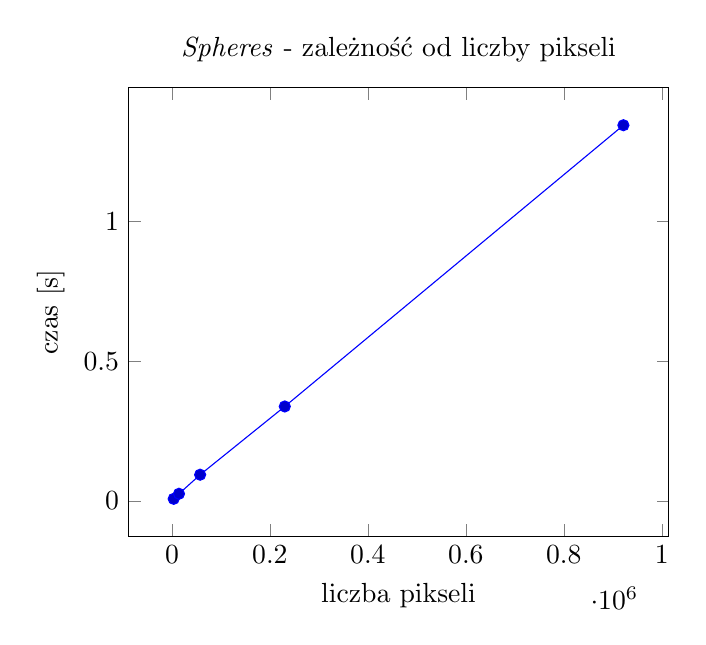
\begin{tikzpicture}
	  \begin{axis}[
	    title=\emph{Spheres} - zależność od liczby pikseli,
	    xlabel=liczba pikseli,
	    ylabel=czas \lbrack s\rbrack,]
	    \addplot coordinates {(3600,0.00764382) (14400,0.0257124) (57600,0.093867) (230400,0.337877) (921600,1.3434)};
	    % if you want the plot to be RED, instead write: \addplot [red,mark=*] coordinates ...
	  \end{axis}
	\end{tikzpicture}
\end{subfigure}
\hspace{2cm}
\begin{subfigure}{.5\textwidth}
		\begin{longtable}{|c|r|} \hline
	    liczba pikseli & \multicolumn{1}{|c|}{spf [s]} \\ \hline
	    3600 (80x45) & 0,008 \\ 
	    14400 (160x90) & 0,026 \\
		57600 (320x180) & 0,094 \\
		230400 (640x360) & 0,338 \\
		921600 (1280x720) & 1,343 \\
		\hline
		\end{longtable}
\end{subfigure}
\end{figure}

\begin{figure}[!htb]
\advance\leftskip-2cm
\begin{subfigure}{.5\textwidth}
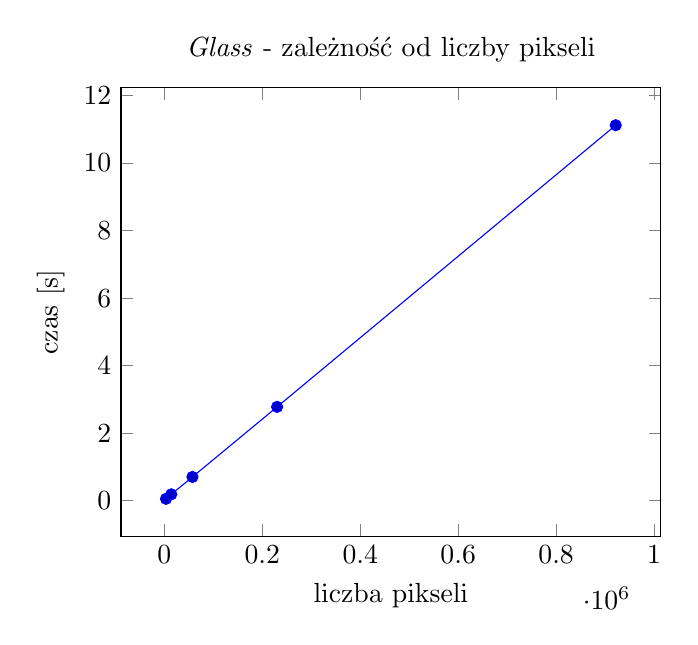
\begin{tikzpicture}
  \begin{axis}[
    title=\emph{Glass} - zależność od liczby pikseli,
    xlabel=liczba pikseli,
    ylabel=czas \lbrack s\rbrack,]
    \addplot coordinates {(3600,0.0567306) (14400,0.191007) (57600,0.705118) (230400,2.77945) (921600,11.1171)};
    % if you want the plot to be RED, instead write: \addplot [red,mark=*] coordinates ...
  \end{axis}
\end{tikzpicture}
\end{subfigure}
\hspace{2cm}
\begin{subfigure}{.5\textwidth}
		\begin{longtable}{|c|r|} \hline
	    liczba pikseli & \multicolumn{1}{|c|}{spf [s]} \\ \hline
	    3600 (80x45) & 0,057 \\ 
	    14400 (160x90) & 0,191 \\
		57600 (320x180) & 0,705 \\
		230400 (640x360) & 2,779 \\
		921600 (1280x720) & 11,117 \\
		\hline
		\end{longtable}
\end{subfigure}
\end{figure}

\begin{figure}[!htb]
\advance\leftskip-2cm
\begin{subfigure}{.5\textwidth}
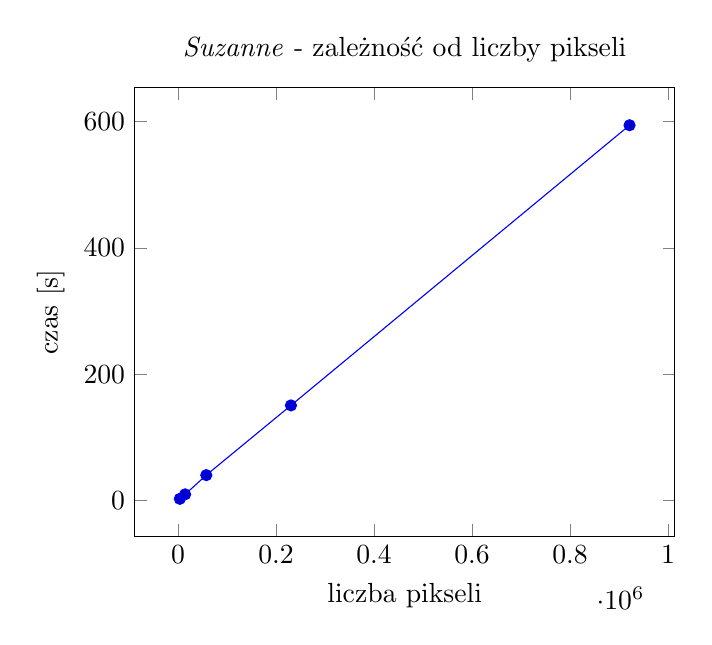
\begin{tikzpicture}
  \begin{axis}[
    title=\emph{Suzanne} - zależność od liczby pikseli,
    xlabel=liczba pikseli,
    ylabel=czas \lbrack s\rbrack,]
    \addplot coordinates {(3600,2.67767) (14400,9.73898) (57600,40.1629) (230400,150.539) (921600,594.091)};
    % if you want the plot to be RED, instead write: \addplot [red,mark=*] coordinates ...
  \end{axis}
\end{tikzpicture}
\end{subfigure}
\hspace{2cm}
\begin{subfigure}{.5\textwidth}
		\begin{longtable}{|c|r|} \hline
	    liczba pikseli & \multicolumn{1}{|c|}{spf [s]} \\ \hline
	    3600 (80x45) & 2,678 \\ 
	    14400 (160x90) & 9,739 \\
		57600 (320x180) & 40,162 \\
		230400 (640x360) & 150,539 \\
		921600 (1280x720) & 594,091 \\
		\hline
		\end{longtable}
\end{subfigure}
\end{figure}


\begin{figure}[!htb]
\advance\leftskip-2cm
\begin{subfigure}{.5\textwidth}
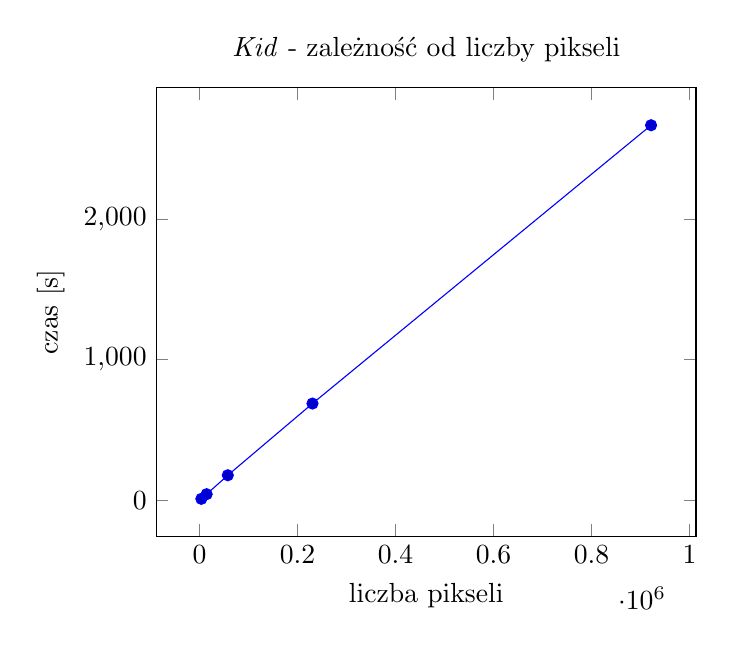
\begin{tikzpicture}
  \begin{axis}[
    title=\emph{Kid} - zależność od liczby pikseli,
    xlabel=liczba pikseli,
    ylabel=czas \lbrack s\rbrack,]
    \addplot coordinates {(3600,11.0737) (14400,44.1641) (57600,178.688) (230400,688.478) (921600,2666.95)};
    % if you want the plot to be RED, instead write: \addplot [red,mark=*] coordinates ...
  \end{axis}
\end{tikzpicture}
\end{subfigure}
\hspace{2cm}
\begin{subfigure}{.5\textwidth}
		\begin{longtable}{|c|r|} \hline
	    liczba pikseli & \multicolumn{1}{|c|}{spf [s]} \\ \hline
	    3600 (80x45) & 11,074 \\ 
	    14400 (160x90) & 44,164 \\
		57600 (320x180) & 178,688 \\
		230400 (640x360) & 688,478 \\
		921600 (1280x720 & 2666,950 \\
		\hline
		\end{longtable}
\end{subfigure}
\end{figure}

Podstawowym wnioskiem, jaki nasuwa się na podstawie otrzymanych wykresów, jest to, że zależność między czasem generowania obrazu a liczbą pikseli jest liniowa, mimo że czas generowania koloru poszczególnych pikseli może być różny. W momencie, w którym promień nie trafi w żaden obiekt, nie zostanie wysłany żaden promień wtórny, co znacząco skraca czas działania algorytmu. Gdy zwiększamy rozmiar obrazu liczba promieni, które trafią w obiekt i takich, które nie trafią nic, rośnie proporcjonalnie do skali powiększenia.

Wiedząc jak zbudowane są sceny, należy zwrócić uwagę na wzrost czasu generowania obrazu w zależności od liczby obiektów. Wykres (!wykres ze stosunkami!) pokazuje, że sceny \emph{Glass} i \emph{Suzzane}, które są podobne do siebie ze względu na budowę (zbudowane są wyłącznie z trójkątów, a generowany obraz jest obrazem zamkniętym - żaden z trójkątów nie wychodzi poza kadr), mają zbliżony stosunek liczby obiektów do czasu generowania klatki. Oznacza to, że ze względu na swoje podobieństwo wzrost liczby obiektów powoduje proporcjonalny wzrost czasu generowania obrazu - jak pokazują pozostałe proste, nie jest to jednak regułą. Dla sceny \emph{Spheres} stosunek liczby obiektów do czasu generowania jest najmniej opłacalny. Jest to spowodowane równomiernym rozrostem drzewa śledzenia promieni - każdy promień trafia w jakiś obiekt, przez co liczba promieni wtórnych rośnie równomiernie. Podobna sytuacja ma miejsce w przypadku sceny \emph{Kid}, jednak tutaj rozrost drzewa jest hamowany przez brak ściany znajdującej się za obserwatorem (część promieni trafia w przestrzeń, co powoduje zmniejszenie liczby promienie wtórnych).

Widzimy, że wzrost czasu generowania obrazu jest w oczywisty sposób zależny od liczby obiektów znajdujących się na scenie, jednak w dużej mierze zależy on również od ich wzajemnego położenia i od położenia obserwatora na scenie (umiejscowienie obserwatora również wpływa na rozrost drzewa, ponieważ to od niego wysyłane są promienie pierwotne). W związku z powyższym przewidzenie ile czasu zajmie generowanie obrazu jest zadaniem trudnym, ale nie niemożliwym - znając wszystkie parametry sceny i algorytmu możemy przewidzieć wersję wydarzeń, w której każdy z promieni napotka na przeszkodę - pesymistyczna złożoność obliczeniowa proponowanego algorytmu (uwzględniającego cienie, dwa rodzaje promieni wtórnych - odbite i załamane) przedstawia się funkcją $T(d,n,o) = (2^d - 1) * o^2 * n$ gdzie:
\\
$d$ - maksymalna głębokość drzewa \\
$o$ - liczba obiektów \\
$n$ - liczba promieni pierwotnych \\ 
\\
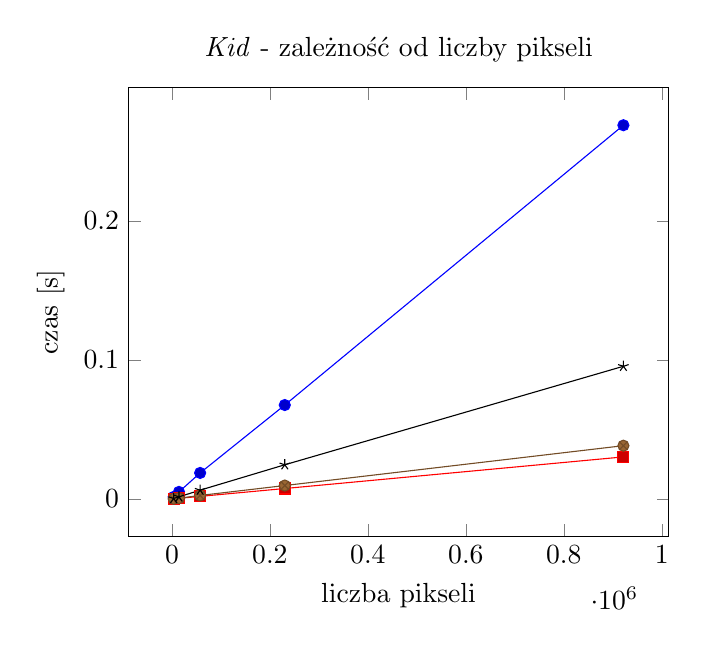
\begin{tikzpicture}
  \begin{axis}[
    title=\emph{Kid} - zależność od liczby pikseli,
    xlabel=liczba pikseli,
    ylabel=czas \lbrack s\rbrack,]
    \addplot coordinates {(3600,0.001528764) (14400,0.00514248) (57600,0.0187734) (230400,0.0675754) (921600,0.26868)};
    \addplot coordinates {(3600,0.000154579) (14400,0.000520455) (57600,0.001921302) (230400,0.007573433) (921600,0.030291826)};
    \addplot coordinates {(3600,0.000172887) (14400,0.000628808) (57600,0.002593162) (230400,0.009719718) (921600,0.038358148)};
    \addplot coordinates {(3600,0.000396253) (14400,0.001580337) (57600,0.006394046) (230400,0.024636012) (921600,0.095432262)};
  \end{axis}
\end{tikzpicture}

\subsection{Zależność czasowa od głębokości drzewa}

W niniejszym podrozdziale zaprezentowano, w jaki sposób zależy czas generowania obrazu od głębokości drzewa śledzenia promieni. Testy zostały przeprowadzone dla kilku różnych ujęć scen zaprezentowanych wyżej (kilka takich samych ujęć dla różnej głębokości drzewa). Obliczenia dotyczące tego punktu nie zostały zrównoleglone. Parametrom niebędącym przedmiotami tego badania zostały arbitralnie przypisane niniejsze wartości:

\begin{itemize}

\item liczba świateł - 1
\item cieniowanie - nie
\item liczba pikseli - 640x360 (230400)
\item użycie drzewa BSP - nie
\item zrównoleglenie - nie

\end{itemize}

\begin{figure}[!htb]
\advance\leftskip-2cm
\begin{subfigure}{.5\textwidth}
\begin{tikzpicture}
  \begin{axis}[
    title=\emph{Spheres} - zależność od głębokości drzewa,
    xlabel=głębokość,
    ylabel=czas \lbrack s\rbrack,]
    \addplot coordinates {(1,0.142384) (2,0.240045) (4,0.444783) (8,0.852983) (16,1.6478)};
    % if you want the plot to be RED, instead write: \addplot [red,mark=*] coordinates ...
  \end{axis}
\end{tikzpicture}
\end{subfigure}
\hspace{2cm}
\begin{subfigure}{.5\textwidth}
		\begin{longtable}{|c|r|} \hline
	    głębokość & \multicolumn{1}{|c|}{spf [s]} \\ \hline
	    1 & 0,142 \\
		2 & 0,240 \\
		4 & 0,445 \\
		8 & 0,853 \\
		16 & 1,648 \\
		\hline
		\end{longtable}
\end{subfigure}
\end{figure}


\begin{figure}[!htb]
\advance\leftskip-2cm
\begin{subfigure}{.5\textwidth}
\begin{tikzpicture}
  \begin{axis}[
    title=\emph{Glass} - zależność od głębokości drzewa,
    xlabel=głębokość,
    ylabel=czas \lbrack s\rbrack,]
    \addplot coordinates {(1,2.16837) (2,2.69988) (4,2.84109) (8,2.86541) (16,2.84629)};
    % if you want the plot to be RED, instead write: \addplot [red,mark=*] coordinates ...
  \end{axis}
\end{tikzpicture}
\end{subfigure}
\hspace{2cm}
\begin{subfigure}{.5\textwidth}
		\begin{longtable}{|c|r|} \hline
	    głębokość & \multicolumn{1}{|c|}{spf [s]} \\ \hline
		1 & 2,168 \\
		2 & 2,670 \\
		4 & 2,841 \\
		8 & 2,865 \\
		16 & 2,846 \\
		\hline
		\end{longtable}
\end{subfigure}
\end{figure}

\begin{figure}[!htb]
\advance\leftskip-2cm
\begin{subfigure}{.5\textwidth}
\begin{tikzpicture}
  \begin{axis}[
    title=\emph{Suzanne} - zależność od głębokości drzewa,
    xlabel=głębokość,
    ylabel=czas \lbrack s\rbrack,]
    \addplot coordinates {(1,129.559) (2,150.077) (4,149.244) (8,151.812) (16,153.429)};
    % if you want the plot to be RED, instead write: \addplot [red,mark=*] coordinates ...
  \end{axis}
\end{tikzpicture}
\end{subfigure}
\hspace{2cm}
\begin{subfigure}{.5\textwidth}
		\begin{longtable}{|c|r|} \hline
	    głębokość & \multicolumn{1}{|c|}{spf [s]} \\ \hline
		1 & 129,559 \\
		2 & 159,077 \\
		4 & 149,244 \\
		8 & 151,812 \\
		16 & 153,429 \\
		\hline
		\end{longtable}
\end{subfigure}
\end{figure}

\begin{figure}[!htb]
\advance\leftskip-2cm
\begin{subfigure}{.5\textwidth}
\begin{tikzpicture}
  \begin{axis}[
    title=\emph{Kid} - zależność od głębokości drzewa,
    xlabel=głębokość,
    ylabel=czas \lbrack s\rbrack,]
    \addplot coordinates {(1,230.193) (2,432.88) (4,843.196) (8,1303.88) (16,1718.51)};
    % if you want the plot to be RED, instead write: \addplot [red,mark=*] coordinates ...
  \end{axis}
\end{tikzpicture}
\end{subfigure}
\hspace{2cm}
\begin{subfigure}{.5\textwidth}
		\begin{longtable}{|c|r|} \hline
	    głębokość & \multicolumn{1}{|c|}{spf [s]} \\ \hline
		1 & 230,193 \\
		2 & 432,880 \\
		4 & 843,196 \\ 
		8 & 1303,880 \\
		16 & 1718,510 \\
		\hline
		\end{longtable}
\end{subfigure}
\end{figure}

Na powyższych wykresach widzimy, że wzrost czasu w zależności od głębokości jest logarytmiczny - jest to spowodowane spadkiem liczby promieni na każdym kolejnym poziomie drzewa (promienie trafiają w próżnię, więc nie są generowane promienie wtórne). Najbardziej wyróżnia się zależność dla sceny \emph{Spheres}, która sprawia wrażenie liniowej. Jest to spowodowane tym, że na tej scenie każdy promień trafia w jakiś obiekt. Teoretycznie funkcje mogłyby rosnąć wykładniczo, ponieważ algorytm dopuszcza generowanie dwóch promieni wtórnych z danego punktu - dzieje się tak, gdy powierzchnia obiektu jest półprzezroczysta - zostaje wysłany promień odbity i promień załamany. W definicji sceny \emph{Spheres} występuje jeden taki obiekt, jednak (jak widać na wykresie) promienie trafiają w niego na tyle rzadko (związane jest to z jego rozmiarami i umiejscowieniem), że nie widzimy tego na wykresie. W przypadku sceny \emph{Kid} każdy obiekt jest w pewnym stopniu przezroczysty, jednak brak ściany pomieszczenia za obserwatorem i tak powoduje spadek promieni wtórnych (jednak jest on wolniejszy niż w przypadku scen \emph{Glass} i \emph{Suzanne}).

\subsection{Zależność czasowa od światła}

W niniejszym podrozdziale zaprezentowano, w jaki sposób zależy czas generowania obrazu od głębokości drzewa śledzenia promieni. Testy zostały przeprowadzone dla kilku różnych ujęć scen zaprezentowanych wyżej, na których losowo rozrzucono zadaną liczbę źródeł światła. Obliczenia dotyczące tego punktu nie zostały zrównoleglone. Parametrom niebędącym przedmiotami tego badania zostały arbitralnie przypisane poniższe wartości:

\begin{itemize}

\item głębokość drzewa śledzenia promieni - 3
\item liczba pikseli - 640x360 (230400)
\item użycie drzewa BSP - nie
\item zrównoleglenie - nie

\end{itemize}

\begin{figure}[!htb]
\advance\leftskip-2cm
\begin{subfigure}{.5\textwidth}
\begin{tikzpicture}
  \begin{axis}[
    title=\emph{Spheres} - zależność od światła,
    xlabel=głębokość,
    ylabel=czas \lbrack s\rbrack,]
    \addplot coordinates {(1,0.251023) (2,0.329837) (4,0.482877) (8,0.786847) (16,1.48653)};
    \addplot coordinates {(1,0.284545) (2,0.318328) (4,0.395992) (8,0.561186) (16,0.561186)};
    % if you want the plot to be RED, instead write: \addplot [red,mark=*] coordinates ...
  \end{axis}
\end{tikzpicture}
\end{subfigure}
\hspace{2cm}
\begin{subfigure}{.5\textwidth}
		\begin{longtable}{|c|r|r|} \hline
		\multirow{2}{*}{liczba świateł} & \multicolumn{2}{|c|}{spf [s]} \\ \cline{2-3}
	    & bez cieni & z cieniami \\ \hline
	    1 & 0,251 & 0,285 \\
	    2 & 0,330 & 0,318 \\
		4 & 0,483 & 0,396 \\
		8 & 0,787 & 0,561 \\
		16 & 1,487 & 1,202 \\
		\hline
		\end{longtable}
\end{subfigure}
\end{figure}


\begin{figure}[!htb]
\advance\leftskip-2cm
\begin{subfigure}{.5\textwidth}
\begin{tikzpicture}
  \begin{axis}[
    title=\emph{Glass} - zależność od światła,
    xlabel=głębokość,
    ylabel=czas \lbrack s\rbrack,]
    \addplot coordinates {(1,2.88157) (2,2.76963) (4,2.78286) (8,2.81478) (16,2.88768)};
    \addplot coordinates {(1,3.27412) (2,3.76403) (4,5.1113) (8,7.44586) (16,10.9446)};
    % if you want the plot to be RED, instead write: \addplot [red,mark=*] coordinates ...
  \end{axis}
\end{tikzpicture}
\end{subfigure}
\hspace{2cm}
\begin{subfigure}{.5\textwidth}
		\begin{longtable}{|c|r|r|} \hline
		\multirow{2}{*}{liczba świateł} & \multicolumn{2}{|c|}{spf [s]} \\ \cline{2-3}
	    & bez cieni & z cieniami \\ \hline
	    1 & 2,881 & 3,274 \\
	    2 & 2,770 & 3,764 \\
		4 & 2,783 & 5,011 \\
		8 & 2,815 & 7,446 \\
		16 & 2,888 & 10,944 \\
		\hline
		\end{longtable}
\end{subfigure}
\end{figure}

\begin{figure}[!htb]
\advance\leftskip-2cm
\begin{subfigure}{.5\textwidth}
\begin{tikzpicture}
  \begin{axis}[
    title=\emph{Suzanne} - zależność od światła,
    xlabel=głębokość,
    ylabel=czas \lbrack s\rbrack,]
    \addplot coordinates {(1,151.408) (2,155.419) (4,162.98) (8,154.59) (16,173.54)};
    \addplot coordinates {(1,146.452) (2,164.65) (4,168.411) (8,201.321) (16,248.212)};
    % if you want the plot to be RED, instead write: \addplot [red,mark=*] coordinates ...
  \end{axis}
\end{tikzpicture}
\end{subfigure}
\hspace{2cm}
\begin{subfigure}{.5\textwidth}
		\begin{longtable}{|c|r|r|} \hline
		\multirow{2}{*}{liczba świateł} & \multicolumn{2}{|c|}{spf [s]} \\ \cline{2-3}
	    & bez cieni & z cieniami \\ \hline
	    1 & 151,408 & 146,452 \\
	    2 & 155,419 & 164,650 \\
		4 & 162,980 & 168,411 \\
		8 & 154,590 & 201,321 \\
		16 & 173,540 & 248,212 \\
		\hline
		\end{longtable}
\end{subfigure}
\end{figure}


\begin{figure}[!htb]
\advance\leftskip-2cm
\begin{subfigure}{.5\textwidth}
\begin{tikzpicture}
  \begin{axis}[
    title=\emph{Kid} - zależność od światła,
    xlabel=głębokość,
    ylabel=czas \lbrack s\rbrack,]
    \addplot coordinates {(1,705.337) (2,716.45) (4,714.296) (8,848.262) (16,853.408)};
    \addplot coordinates {(1,1040.56) (2,1435.52) (4,2330.47) (8,3904.24) (16,6871.04)};
    % if you want the plot to be RED, instead write: \addplot [red,mark=*] coordinates ...
  \end{axis}
\end{tikzpicture}
\end{subfigure}
\hspace{2cm}
\begin{subfigure}{.5\textwidth}
		\begin{longtable}{|c|r|r|} \hline
		\multirow{2}{*}{liczba świateł} & \multicolumn{2}{|c|}{spf [s]} \\ \cline{2-3}
	    & bez cieni & z cieniami \\ \hline
	    1 & 705,337 & 1040,560 \\
	    2 & 716,45 & 1435,520 \\
		4 & 714,296 & 2330,470 \\
		8 & 848,262 & 3904,240 \\
		16 & 853,408 & 6871,040 \\
		\hline
		\end{longtable}
\end{subfigure}
\end{figure}

Z powyższych wykresów wynika, że wpływ liczby źródeł światła na czas generowania obrazu jest znaczny, zwłaszcza w przypadku, w którym śledzimy promień od punktu przecięcia promienia z obiektem do źródła światła (w celu sprawdzenia czy punkt znajduje się w cieniu). Uwzględnienie cieni wymaga przeglądu wszystkich obiektów tak długo, aż nie znajdzie się jakiś między punktem a źródłem światła. W najgorszym przypadku, czyli takim, w którym nic nie rzuca cienia, musimy przejrzeć wszystkie obiekty. W przypadku skomplikowanych scen znacznie wydłuża to czas generowania obrazu (zwłaszcza, że należy to zrobić dla każdego ze źródeł światła - stąd liniowy wzrost czasu generowania obrazu). Wyjątek stanowi scena \emph{Spheres} zawierająca niewielką liczbę obiektów. W sytuacji, w której jakiś obiekt znajduje się w cieniu, nie musimy dla danego punktu wyliczać koloru korzystając z \emph{Modelu Phonha} <!ROZDZIAŁ!> - liczy się tylko światło otoczenia. W związku z tym przy niewielkiej liczbie obiektów koszt jego szukania jest niewielki. Oszczędzamy czas procesora dzięki temu, że nie musimy korzystać ze skomplikowanego modelu światła - paradoksalnie bardziej realistyczny obraz generuje się szybciej.

\subsection{Zależność czasowa od zrównoleglenia}

W niniejszym podrozdziale pokazano, w jakim stopniu zrównoleglenie pozwala na przyspieszenie generowania obrazu. Testy zostały przeprowadzone dla pięciu różnych ziarnistości podziału obrazu (ziarnistość zadania) i dla trzech różnych ilości zaangażowanych procesorów. Testy dla pięciu procesorów zostały przeprowadzone na jednej maszynie, dla dziesięciu na dwóch i dla piętnastu na trzech (wartość podana w tabelach uwzględnia tylko węzły wykonawcze). Każdy z komputerów był maszyną wirtualną, której udostępniono 6 procesorów wirtualnych. Połączenia pomiędzy komputerami były realizowane poprzez technologię \emph{Fast Ethernet}. W dolnej części tabel z wynikami podano ilokrotnie maksymalnie przyspieszyły obliczenia względem podejścia niezrównoleglonego (stosunek czasu obliczeń algorytmu wykonującego się na jednym procesorze do minimalnego czasy otrzymanego w teście). Czas generowania obrazu z wykorzystaniem pojedynczego procesora został wyliczony na nowo i nie ma nic wspólnego z czasami podanymi uprzednio. Powodem takiego podejścia jest to, że testy omówione wyżej były wykonywane na fizycznej maszynie o innej specyfikacji. Parametrom niebędącym przedmiotami tego badania zostały arbitralnie przypisane niniejsze wartości:

\begin{itemize}

\item liczba świateł - 1
\item cieniowanie - tak
\item głębokość drzewa śledzenia promieni - 3
\item użycie drzewa BSP - nie

\end{itemize}

%%%%%%%%%%%%%%%%%%%%%%%%%%%%%%%%%%%%%%%%%%%%%%%%%%%
\begin{figure}[!htb]
\advance\leftskip-2cm
	\begin{subfigure}{.5\textwidth}
	\begin{tikzpicture}
	  \begin{axis}[
	    title=\emph{Spheres} - zależność od zrównoleglenia (640x360),
	    xlabel=głębokość,
	    ylabel=czas \lbrack s\rbrack,]
	    \addplot coordinates {(16,0.179093) (36,0.170406) (64,0.206508) (100,0.213478) (144,0.252288)};
	    \addplot coordinates {(16,0.0881486) (36,0.0854354) (64,0.103843) (100,0.145735) (144,0.218693)};
	    \addplot coordinates {(16,0.0619428) (36,0.063786) (64,0.0976417) (100,0.145701) (144,0.217703)};
	    \addplot coordinates {(16,0.279) (36,0.279) (64,0.279) (100,0.279) (144,0.279)};
	  \end{axis}
	\end{tikzpicture}
	\end{subfigure}
	\hspace{2cm}
	\begin{subfigure}{.5\textwidth}
	\begin{tikzpicture}
	  \begin{axis}[
	    title=\emph{Spheres} - zależność od zrównoleglenia (640x360),
	    xlabel=głębokość,
	    ylabel=czas \lbrack s\rbrack,]
	    \addplot coordinates {(1,0.279) (4,0.170406) (9,0.0854354) (14,0.063786)};
	  \end{axis}
	\end{tikzpicture}
\end{subfigure}
\end{figure}

\begin{figure}[!htb]
\begin{longtable}{|c|r|r|r|} \hline
	    \multirow{2}{*}{liczba fragmentów} & \multicolumn{3}{|c|}{spf [s]} \\ \cline{2-4}
	 	& 4 proc. & 9 proc. & 14 proc. \\ \hline
	    16 & 0,179 & 0,088 & 0,062 \\ 
	    36 & 0,170 & 0,086 & 0,064 \\
		64 & 0,207 & 0,104 & 0,098 \\
		100 & 0,213 & 0,146 & 0,146 \\
		144 & 0,252 & 0,219 & 0,218 \\ \hline
		max przysp. & 1,640 & 3,270 & 4,500 \\
		\hline
\end{longtable}
\end{figure}

%%%%%%%%%%%%%%%%%%%%%%%%%%%%%%%%%%%%%%%%%%%%%%%%%%%%%%%%%%%%%%%%
\begin{figure}[!htb]
\advance\leftskip-2cm
	\begin{subfigure}{.5\textwidth}
	\begin{tikzpicture}
	  \begin{axis}[
	    title=\emph{Glass} - zależność od zrównoleglenia (640x360),
	    xlabel=głębokość,
	    ylabel=czas \lbrack s\rbrack,]
	    \addplot coordinates {(16,1.09964) (36,1.05298) (64,1.03611) (100,1.02236) (144,1.05367)};
	    \addplot coordinates {(16,0.742264) (36,0.548189) (64,0.513832) (100,0.507293) (144,0.544521)};
	    \addplot coordinates {(16,0.479671) (36,0.407425) (64,0.311017) (100,0.322993) (144,0.344262)};
	    \addplot coordinates {(16,2.401) (36,2.401) (64,2.401) (100,2.401) (144,2.401)};
	    % if you want the plot to be RED, instead write: \addplot [red,mark=*] coordinates ...
	  \end{axis}
	\end{tikzpicture}
	\end{subfigure}
		\hspace{2cm}
		\begin{subfigure}{.5\textwidth}
	\begin{tikzpicture}
	  \begin{axis}[
	    title=\emph{Spheres} - zależność od zrównoleglenia (640x360),
	    xlabel=głębokość,
	    ylabel=czas \lbrack s\rbrack,]
	    \addplot coordinates {(1,2.401) (4,1.02236) (9,0.507293) (14,0.311017)};
	  \end{axis}
	\end{tikzpicture}
	\end{subfigure}
\end{figure}

\begin{figure}[!htb]
\begin{longtable}{|c|r|r|r|} \hline
	    \multirow{2}{*}{liczba fragmentów} & \multicolumn{3}{|c|}{spf [s]} \\ \cline{2-4}
	 	& 4 proc. & 9 proc. & 14 proc. \\ \hline
	    16 & 1,100 & 0,742 & 0,480 \\ 
	    36 & 1,053 & 0,548 & 0,407 \\
		64 & 1,036 & 0,514 & 0,311 \\
		100 & 1,022 & 0,507 & 0,323 \\
		144 & 1,053 & 0,545 & 0,344 \\ \hline
		max przysp. & 2,350 & 4,730 & 7,720  \\
		\hline
\end{longtable}
\end{figure}

%%%%%%%%%%%%%%%%%%%%%%%%%%%%%%%%%%%%%%%%%%%%%%%%%%%%%%%%%%%%%%%%
\begin{figure}[!htb]
\advance\leftskip-2cm
	\begin{subfigure}{.5\textwidth}
	\begin{tikzpicture}
	  \begin{axis}[
	    title=\emph{Suzanne} - zależność od zrównoleglenia (640x360),
	    xlabel=głębokość,
	    ylabel=czas \lbrack s\rbrack,]
	    \addplot coordinates {(16,205.605) (36,206.972) (64,209.42) (100,217.794) (144,205.472)};
	    \addplot coordinates {(16,75.4728) (36,70.136) (64,71.2841) (100,70.7879) (144,71.007)};
	    \addplot coordinates {(16,52.8091) (36,37.398) (64,39.9895) (100,37.832) (144,37.0606)};
	    \addplot coordinates {(16,336.1612) (36,336.1612) (64,336.1612) (100,336.1612) (144,336.1612)};
	  \end{axis}
	\end{tikzpicture}
	\end{subfigure}
	\hspace{2cm}
		\begin{subfigure}{.5\textwidth}
	\begin{tikzpicture}
	  \begin{axis}[
	    title=\emph{Spheres} - zależność od zrównoleglenia (640x360),
	    xlabel=głębokość,
	    ylabel=czas \lbrack s\rbrack,]
	    \addplot coordinates {(1,336.1612) (4,205.472) (9,70.136) (14,37.0606)};
	  \end{axis}
	\end{tikzpicture}
	\end{subfigure}
\end{figure}

\begin{figure}[!htb]
\begin{longtable}{|c|r|r|r|} \hline
	    \multirow{2}{*}{liczba fragmentów} & \multicolumn{3}{|c|}{spf [s]} \\ \cline{2-4}
	 	& 4 proc. & 9 proc. & 14 proc. \\ \hline
	    16 & 205,605 & 75,473 & 52,809 \\ 
	    36 & 206,972 & 70,136 & 37,398 \\
		64 & 209,420 & 71,284 & 39,900 \\
		100 & 217,794 & 70,788 & 37,383 \\
		144 & 205,472 & 71,007 & 37,061 \\ \hline
		max przysp. & 1,640 & 4,790 & 9,070 \\
		\hline
\end{longtable}
\end{figure}

%%%%%%%%%%%%%%%%%%%%%%%%%%%%%%%%%%%%%%%%%%%%%%%%%%%%%%%%%%%%%%%%%
\begin{figure}[!htb]
\advance\leftskip-2cm
	\begin{subfigure}{.5\textwidth}
	\begin{tikzpicture}
	  \begin{axis}[
	    title=\emph{Kid} - zależność od zrównoleglenia (640x360),
	    xlabel=głębokość,
	    ylabel=czas \lbrack s\rbrack,]
	    \addplot coordinates {(16,1634.56) (36,1624.21) (64,1616.771) (100,1620.153) (144,1647.817)};
	    \addplot coordinates {(16,647.817) (36,565.67) (64,567.067) (100,563.411) (144,575.474)};
	    \addplot coordinates {(16,439.232) (36,375.321) (64,318.538) (100,311.411) (144,306.143)};
	    \addplot coordinates {(16,2677.71) (36,2677.71) (64,2677.71) (100,2677.71) (144,2677.71)};
	  \end{axis}
	\end{tikzpicture}
	\end{subfigure}
		\hspace{2cm}
	\begin{subfigure}{.5\textwidth}
	\begin{tikzpicture}
	  \begin{axis}[
	    title=\emph{Spheres} - zależność od zrównoleglenia (640x360),
	    xlabel=głębokość,
	    ylabel=czas \lbrack s\rbrack,]
	    \addplot coordinates {(1,2677.71) (4,1616.771) (9,563.411) (14,306.143)};
	  \end{axis}
	\end{tikzpicture}
	\end{subfigure}
\end{figure}
%%%%%%%%%%%%%%%%%%%%%%%%%%%%%%%%%%%%%%%%%%%%%%%%%%%%%%%%%%%%%%%%%%%


\begin{figure}[!htb]
\begin{longtable}{|c|r|r|r|} \hline
	    \multirow{2}{*}{liczba fragmentów} & \multicolumn{3}{|c|}{spf [s]} \\ \cline{2-4}
	 	& 4 proc. & 9 proc. & 14 proc. \\ \hline
	    16 & 1634,560 & 647,817 & 439,232 \\ 
	    36 & 1624,210 & 565,670 & 375,321 \\
		64 & 1616,771 & 567,067 & 318,538 \\
		100 & 1620,153 & 563,411 & 311,411 \\
		144 & 1639,121 & 575,474 & 306,143 \\ \hline
		max przysp. & 1,660 & 4,750 & 8,750  \\
		\hline
\end{longtable}
\end{figure}

Najważniejszym wnioskiem płynącym z powyższych badań jest to, że wraz ze wzrostem liczby węzłów czas generowania maleje logarytmicznie. Oznacza to, że w pewnym momencie zwiększania rozmiarów klastra, nie uzyskamy żadnego przyspieszenia obliczeń. Jest to wniosek zgodny z oczekiwaniami - maksymalna liczba komputerów, której moc obliczeniową można by wykorzystać, nie będzie większa od liczby pikseli obrazu (przynajmniej dla tej metody zrównoleglenia). Górne ograniczenie rozmiarów klastra (dla zadanej wielkości obrazu) jest oczywiście niższe ze względu na czas potrzebny do przesłania informacji pomiędzy węzłami.

Zastanówmy się teraz nad optymalną ziarnistością zadania (liczbą wycinków obrazu). Najciekawiej prezentuje się wykres dotyczący sceny \emph{Spheres} - wraz ze wzrostem liczby wycinków, drastycznie spada wydajność klastra. Dzieje się tak dlatego, ponieważ więcej czasu zajmuje przesyłanie danych pomiędzy węzłami niż rzeczywiste obliczenia. Na pozostałych wykresach liczba wycinków zdaje się nie mieć takiego znaczenia, jednak jest to spowodowane zastosowaną skalą. Wg. danych z tabeli <!numer tabeli!>, optymalną liczba wycinków dla 14 procesów oscyluje wokół wartości 64. Dla pozostałych scen czas generowania klatki spada wraz ze wzrostem ziarnistości. Warto zwrócić uwagę, że dla 14 procesów czas działania algorytmu dla 16 fragmentów jest najdłuższy - jest to spowodowane tym, że po policzeniu pierwszej partii zadań wiele węzłów pozostaje bezczynnych. Dane pokazują również, że optymalna ziarnistość zmienia się wraz ze zmianą rozmiaru klastra.

\subsection{Wykorzystanie drzewa BSP}

W niniejszym podrozdziale pokazano, w jakim stopniu wykorzystanie drzewa BSP pozwala na przyspieszenie generowania obrazu.  W dolnej części tabel z wynikami podano ilokrotnie maksymalnie przyspieszyły obliczenia względem podejścia niezrównoleglonego (stosunek czasu obliczeń algorytmu wykonującego się na jednym procesorze do minimalnego czasy otrzymanego w teście) oraz czas budowy drzewa BSP.
Parametrom niebędącym przedmiotami tego badania zostały arbitralnie przypisane poniższe wartości:

\begin{itemize}

\item głębokość drzewa śledzenia promieni - 3
\item liczba pikseli - 640x360 (230400)
\item użycie drzewa BSP - nie
\item liczba świateł - 1
\item cieniowanie - tak
\item liczba węzłów wykonawczych - 14 

\end{itemize}



\begin{figure}[!htb]
\advance\leftskip-2cm
	\begin{subfigure}{.5\textwidth}
	\begin{tikzpicture}
	  \begin{axis}[
	    title=\emph{Glass} - BSP 0.107058,
	    xlabel=głębokość,
	    ylabel=czas \lbrack s\rbrack,]
	    \addplot coordinates {(16,5.21946) (36,3.8034) (64,3.57917) (100,3.40521) (144,3.53286)};
	    \addplot coordinates {(16,4.99529) (36,2.71377) (64,2.48849) (100,2.2844) (144,2.33781)};
	  \end{axis}
	\end{tikzpicture}
	\end{subfigure}
	\hspace{2cm}
	\begin{subfigure}{.5\textwidth}
	\begin{longtable}{|c|r|r|} \hline
	    \multirow{2}{*}{liczba fragmentów} & \multicolumn{2}{|c|}{spf [s]} \\ \cline{2-3}
	    & brak bryły ot. & z bryłą ot. \\ \hline
	    16 & 5,219 & 4,995 \\ 
	    36 & 3,803 & 2,714 \\
		64 & 3,579 & 2,488 \\
		100 & 3,405 & 2,284 \\
		144 & 3,533 & 2,338 \\ \hline
		max przysp. & 0,700 & 1,050 \\ \hline
		czas gen. drzewa [s] &  \multicolumn{2}{|c|}{0,107} \\ \hline
	\end{longtable}
\end{subfigure}
\end{figure}
\pagebreak
\begin{figure}[!htb]
\advance\leftskip-2cm
	\begin{subfigure}{.5\textwidth}
	\begin{tikzpicture}
	  \begin{axis}[
	    title=\emph{Suzzane} - BSP 317.279,
	    xlabel=głębokość,
	    ylabel=czas \lbrack s\rbrack,]
	    \addplot coordinates {(16,14.3402) (36,10.0665) (64,9.23015) (100,8.29159) (144,8.06655)};
	    \addplot coordinates {(16,16.6061) (36,9.51138) (64,8.03645) (100,7.68939) (144,8.03335)};
	  \end{axis}
	\end{tikzpicture}
	\end{subfigure}
	\hspace{2cm}
	\begin{subfigure}{.5\textwidth}
	\begin{longtable}{|c|r|r|} \hline
	    \multirow{2}{*}{liczba fragmentów} & \multicolumn{2}{|c|}{spf [s]} \\ \cline{2-3}
	    & brak bryły ot. & z bryłą ot. \\ \hline
	    16 & 14,340 & 16,606 \\ 
	    36 & 10,067 & 9,511 \\
		64 & 9,230 & 8,036 \\
		100 & 8,292 & 7,689 \\
		144 & 8,067 & 8,033 \\ \hline
		max przysp. & 41,670 & 43,710 \\ \hline
		czas gen. drzewa [s] &  \multicolumn{2}{|c|}{317,279} \\ \hline
	\end{longtable}
\end{subfigure}
\end{figure}

Metoda śledzenia promieni wykorzystująca drzewo BSP pozwoliła na zmniejszenie czasu generowania obliczeń sceny \emph{Suzanne} do kilku sekund. Początkowy (i co ważne jednorazowy) koszt budowy drzewa przyniósł pożądane rezultaty. Inaczej ma się sytuacja w przypadku sceny \emph{Glass}, która, jak wynika z powyższych danych, jest przypadkiem sceny, dla której korzystanie z drzewa BSP jest nieopłacalne - nie dość, że musieliśmy ponieść koszt związany z jego budową, to jeszcze generowanie kolejnych klatek trwa dłużej niż w przypadku algorytmu niezrównoleglonego. Jakie cechy musi posiadać scena, żeby korzystanie z drzewa BSP było opłacalne i w jaki sposób możemy poprawić jego działanie?

Podstawową problemem sceny \emph{Glass} jest duża liczba promieni pierwotnych, które w nic nie trafiają. Biorąc pod uwagę, że obserwator widzi całą scenę, to większość płaszczyzn dzielących jest przez te promienie przecinane (w zależności od ich nachylenia). W takiej sytuacji algorytm szukania najbliższego obiektu więcej czasu spędza na trawersowaniu drzewa niż miałoby to miejsce w przypadku przeglądu zupełnego - odwiedzi on większość węzłów drzewa. Kolejnym czynnikiem mogącym powodować problem jest wzajemne ułożenie wielokątów na scenie. W sytuacji, w której tworzą one zbiór wypukły, wybieranie płaszczyzny dzielącej spośród tych wyznaczanych przez te wielokąty, sprawia, że żadna z nich nie podzieli przestrzeni. Częściowym rozwiązaniem tego problemu jest szukanie kandydatów na płaszczyzny dzielące nie tylko wśród takich, które pokrywają się w wielokątami sceny, ale też wśród płaszczyzn prostopadłych do tych wieloboków - takie podejście zostało zaimplementowane w testowanym algorytmie.

W celu polepszenia wydajności drzew BSP należy się skupić na czterech elementach: wprowadzeniu brył otaczających (redukcja liczby promieni nietrafiających w żaden obiekt, dla których trzeba by było przeprowadzać testy z wykorzystaniem drzewa BSP), poszukiwaniu lepszej metody wyboru kandydatów na płaszczyzny dzielące, ulepszeniu funkcji oceny płaszczyzny (np. zastosowanie funkcji SAH - !ROZDZIAŁ!), lub poprawie algorytmu trawersowania drzewa.

W celu pokazania, w jakim stopniu wprowadzenie brył otaczających może poprawić rezultaty, testowane sceny zostały zamknięte w prostopadłościanach. Jak widać na wykresie (!wykres szklanka!) zysk czasowy wynikający z zastosowania bryły otaczającej jest znaczący, jednak czas generowania obrazu ciągle jest lepszy dla przeglądu zupełnego. W przypadku \emph{Suzanne} różnica zdaje się być niewielka. Wynika to z położenia obserwatora - w sytuacji, w której znajduje się on blisko obiektu (stosunkowo mało promieni pierwotnych nie trafia w nic), zastosowanie bryły otaczającej w kształcie prostopadłościanu redukuje niewielką liczbę testów. Gdyby obserwator zaczął się oddalać od obiektu, to czas generowania obrazu z wykorzystaniem drzewa BSP by rósł, jednak dzięki wykorzystaniu bryły otaczającej tendencja się odwróci. Niżej przedstawiono mapy cieplne obrazujące które piksele liczyły się najdłużej. Im jaśniejszy obszar tym jego wygenerowanie zajęło więcej czasu. Szum pojawiający się na obrazach jest najprawdopodobniej spowodowany przełączaniem się procesów.

\begin{figure}[h!]
\centering
  \caption{Przegląd zupełny}
  \includegraphics[width=15cm]{normal.png}
\end{figure}

Na powyższej mapie cieplnej widzimy, że najwięcej czasu algorytm spędził na generowaniu pikseli zawierających model.

\begin{figure}[h!]
\centering
  \caption{Brak wykorzystanie bryły otaczającej}
  \includegraphics[width=15cm]{noaabb.png}
\end{figure}

W przypadku zastosowania drzewa BSP ciężar obliczeń spadł na otoczenie modelu a nie na sam model. Powyższy obraz w interesujący sposób przedstawia płaszczyzny dzielące przestrzeń. Elementy znajdujące się za większą liczbą płaszczyzn są jaśniejsze. 

\begin{figure}[h!]
\centering
  \caption{Z wykorzystaniem bryły otaczającej}
  \includegraphics[width=15cm]{aabb.png}
\end{figure}

Zastosowanie bryły otaczającej sprawia, że czas liczenia promieni nie trafiających w żaden obiekt maleje właściwie do zera (koszt badania przecięcia promienia z bryłą otaczającą). Wbrew temu, co może sugerować powyższy obraz, każda ze ścian bryły otaczającej jest styczna do modelu - wrażenie, że jest inaczej powoduje rzut perspektywiczny (elementy, które są bliżej nas, zdają się być większe). Nie byłoby, tak gdyby został zastosowany rzut prosty.

Na podstawie powyższych informacji można wywnioskować, że zastosowanie brył otaczających, które lepiej przylegałyby do modeli, zmniejszy czas wykonywania obliczeń. Dodatkowo, chcąc wprowadzić funkcję SAH niezbędne, jest zamknięcie całej sceny w bryle, ponieważ ta wymaga liczenia objętości podprzestrzeni (musi więc istnieć jakieś ograniczenie). Naturalnym rozwinięciem wydaje się również wprowadzenie hierarchii brył otaczających - na podstawie powyższej analizy zdaje się, że każdy integralny i nieruchomy obiekt powinien być najpierw zamknięty w bryle, a następnie dzielony z wykorzystaniem drzewa BSP. Rozwiązania hybrydowe są szeroko stosowane w grafice, zwłaszcza, że drzewo BVH ma tą wyższość nad drzewem BSP, że przemieszczanie się obiektów nie wymaga przebudowania go całego.

\section{Przykładowe obrazy}


\begin{figure}[htb!]
\centering
  \caption{Spheres}
  \includegraphics[width=\textwidth]{psycho.png}
\end{figure}


\begin{figure}[htb!]
\centering
  \caption{Spheres}
  \includegraphics[width=\textwidth]{mirror.png}
\end{figure}


\begin{figure}[htb!]
\centering
  \caption{Spheres}
  \includegraphics[width=\textwidth]{glasssphere.png}
\end{figure}

\begin{figure}[htb!]
\centering
  \caption{Spheres}
  \includegraphics[width=\textwidth]{light8s.png}
\end{figure}


\begin{figure}[htb!]
\centering
  \caption{Spheres}
  \includegraphics[width=\textwidth]{water.png}
\end{figure}

\begin{figure}[htb!]
\centering
  \caption{Spheres}
  \includegraphics[width=\textwidth]{mask.png}
\end{figure}



\chapter{Podsumowanie}
Podstawowym celem tej pracy było zbadanie, czy metoda śledzenia promieni ma rację bytu w interaktywnych aplikacjach graficznych. By uzyskać odpowiedź na to pytanie przeprowadzono szereg testów pokazujących między innymi, w jaki sposób definicja sceny, której dwuwymiarowa wizualizacja ma się pojawić przed oczami użytkownika, wpływa na czas generowania obrazu. Dzięki nim dowiedzieliśmy się, w jaki sposób czynniki takie jak rozmiar obrazu, liczba świateł, głębokość drzewa wpływają na szybkość obliczeń. Taka wiedza pozwala na umiejętne minimalizowanie czasu potrzebnego na generowanie realistycznych grafik przy niewielkim wpływie na jakość obrazu.

Przejdźmy do omówienia wyników zrównoleglenia algorytmu. Dzięki niemu możliwe było uzyskanie ok. 16 klatek na sekundę przy najmniej skomplikowanej scenie (\emph{Spheres}), która mimo swojej prostoty i tak była bardzo efektowna. Dla większej liczby obiektów znajdujących się na scenie rezultaty nie były wystarczające (mimo maksymalnego przyspieszenia sięgającego 900\%) - klatka dla sceny \emph{Glass} generowała się ok. 0,3 sekundy, dla \emph{Suzanne} 37 sekund, a dla \emph{Room} ok. 5 min. Takie czasy są niedopuszczalne. W ramach badań nad możliwością przyspieszenia obliczeń generowania obrazu zostało przetestowane drzewo BSP. Okazuje się, że pozwala ono w niektórych sytuacjach (dokładnie w jakich zostało opisane w punkcie 7.1.5) na znaczne przyspieszenie obliczeń (czas generowania obrazu na podstawie sceny \emph{Suzanne} spadł do 8 sekund), jednak, jak pokazuje alternatywny, ,,zły'' przykład \emph{Glass}, potrafi również pogorszyć wydajność. Walką z tego typu sytuacjami może być zmiana strategi podziału przestrzeni na \emph{SAH} (punkt 2.2.4), lub zastosowanie brył otaczających. Istnieje możliwość podejścia hybrydowego, które wykorzystywałoby zalety zarówno drzew BSP jak i drzew BVH - w celu implementacji takiego podejścia należy dokładnie zbadać zachowanie drzew BVH, a następnie próbować łączyć ze sobą oba rozwiązania (prawdopodobnie modyfikując książkowe zachowanie jednego i drugiego). Propozycją, która nie jest uzasadniona żadnymi badaniami a czystą intuicją, jest zamykanie integralnych, nieruchomych (drzewa BVH nie potrzebują przebudowy w przypadku przemieszczenia się obiektów) modeli w bryłach otaczających, a następnie podział tych brył drzewem BSP - takie rozwiązanie powinno zmniejszyć negatywny wpływ wad drzewa BSP.

Czy metoda śledzenia promieni może być wykorzystywana w aplikacjach interaktywnych? Uważam, że tak - badania, jakie zostały przeprowadzone, pozwalają przypuszczać, że gdyby do zrównoleglenia obliczeń był wykorzystywany koprocesor graficzny (\emph{GPU}), to stopień przyspieszania powinien być wystarczający do budowania np. prostych gier komputerowych opartych na tym algorytmie. Możliwość dalszych optymalizacji, które powinny poprawić rezultaty, zdaje się potwierdzać tę hipotezę. Ciekawa wydaje się również możliwość zbudowania klastra obliczeniowego opartego o karty graficzne. Czy takie rozwiązanie będzie efektywne, mogłyby wyjaśnić dopiero dalsze badania prowadzone w tym kierunku.

%\bibliographystyle{plain}
%\bibliography{bibliography}{}
%\addcontentsline{toc}{chapter}{Bibliografia}
\begin{thebibliography}{99}

\bibitem{bspfaq}
	BSP FAQ: \\
	ftp://ftp.sgi.com/other/bspfaq/faq/bspfaq.html, 03.11.2017

\bibitem{wikiPar}
	Czech Z. J. 
	\emph{Wprowadzenie do obliczeń równoległych},
	Wydawnictwo Naukowe PWN, 2013
	
\bibitem{bvhvsoctee}
	Dievald T., http://thomasdiewald.com/blog/?p=1488, 11.08.2017

\bibitem{dunn02}
  Dunn F., Parberry I.,
  \emph{3D Math Primer for Graphics and Game Development}.
  Wordware Publishing, Inc.
  2002.

\bibitem{trees}
	Ericson Christer,
	\emph{Real-Time Collision Detection},
	CRC Press, 2005
	
\bibitem{falski2004}
	Falski M. 
	\emph{Przegląd modeli oświetlenia w grafice komputerowej}
	Praca magisterska pod kierunkiem dr A. Łukaszewskiego,
	Uniwersytet Wrocławski,
	2004

\bibitem{foley95}
  Foley J. D.  i in.
  \emph{Wprowadzenie do Grafiki Komputerowej}.
  tłum. J. Zabrodzki,
  WNT, Warszawa
  1995.
  
\bibitem{octree1}
	Glassner A. S. ,
	\emph{Space Subdivision for Fast Ray Tracing},
	University of North Carolina at Chapel Hill,
	1984 
	
\bibitem{sah1}
	Kammaje R. P., Mora B.,
	\emph{A Study of Restricted BSP Trees for Ray Tracing}
	University of Wales Swansea,
	2007
	
\bibitem{mpich}
	Dokumentacja MPICH | High-Performance Portable MPI: \\
	https://www.mpich.org/, 03.07.2017 
	
\bibitem{qt}
	Dokumentacja biblioteki Qt: \\
	http://wiki.qt.io, 09.09.2017
  
\bibitem{suffern2007}
	Suffern K. 
	\emph{Ray Tracing from the Ground Up}.
	A K Peters, Ltd.
	Wellesley, Massachusetts,
	2007.
	
\bibitem{octree2}
	Samet H.,
	\emph{Implementing Ray Tracing with Octrees and Neighbor Finding},
	University of Maryland,
	Collage Park, 1989	
	
\bibitem{scratch}
	StrachPixel 2.0:
	https://www.scratchapixel.com, 27.09.2017
		
\bibitem{bspvskd}
	Vinkler T., Havran V., Bittner J.,
	\emph{Bounding Volume Hierarchies versus Kd-trees on Contemporary Many-Core Architectures},
	Marsyk University, Czech Technical University in Praque, 2016 
	

\bibitem{sah2}
	Wald I.,
	\emph{Realtime Ray Tracing and Interactive Global Illumination},
	Computer Graphics Group, Saarland University Saarbrucken, Germany,
	2004

\bibitem{snellius}
	Walker J., Halliday D., Resnick. R,
	\emph{Podstawy Fizyki}, str. 23,
	PWN, Warszawa,
	2016.

\bibitem{wikiMoll}
	Wikipedia, Wolna Encyklopedia:\\ 
	https://en.wikipedia.org/wiki/Moller–Trumbore\_intersection\_algorithm, 15.09.2017
	
\bibitem{bvhvskd2}
	Zlatuska M., Havran V. 
	\emph{Ray Tracing on a GPU with CUDA –
Comparative Study of Three Algorithms},
	Czech Technical University in Praque,
	2010
	
\bibitem{zuk2008}
	Żukowski R.,
	\emph{Automatyczna dekompozycja sceny 3D na portale i sektory}
	Praca magisterska pod kierunkiem dr A. Łukaszewskiego,
	Uniwersytet Wrocławski,
	2008
	
\bibitem{gpipe}
	Internetowa encyklopedia na temat OpenGL: \\
	https://www.khronos.org/opengl/wiki/Rendering\_Pipeline\_Overview, 11.10.2017
	
\end{thebibliography}


\end{document}